\documentclass[a4paper,11pt]{book}
%\documentclass[a4paper,twoside,11pt,titlepage]{book}
\usepackage{listings}
\usepackage[utf8]{inputenc}
\usepackage[spanish]{babel}

% para poner notas:
\usepackage[colorinlistoftodos,prependcaption,textsize=tiny]{todonotes}

\usepackage[acronym]{glossaries}
\makeglossaries
%\usepackage{titlesec}
%\usepackage{pailatino}

\usepackage{color}

\decimalpoint
\usepackage{dcolumn}
\newcolumntype{.}{D{.}{\esperiod}{-1}}
\makeatletter
\addto\shorthandsspanish{\let\esperiod\es@period@code}
\makeatother


%\usepackage[chapter]{algorithm}
\RequirePackage{verbatim}
%\RequirePackage[Glenn]{fncychap}
\usepackage{fancyhdr}
\usepackage{graphicx}
\usepackage{afterpage}

\usepackage{longtable}

\usepackage[pdfborder={000}]{hyperref} %referencia

% ********************************************************************
% Re-usable information
% ********************************************************************
\newcommand{\myTitle}{Diseño e implementación de red inteligente autoconfigurable\xspace}
\newcommand{\myDegree}{Grado en ...\xspace}
\newcommand{\myName}{Javier Sáez de la Coba (alumno)\xspace}
\newcommand{\myProf}{Juan José Ramos Muñoz (Tutor)\xspace}
\newcommand{\myOtherProf}{\xspace}
%\newcommand{\mySupervisor}{Put name here\xspace}
\newcommand{\myFaculty}{Escuela Técnica Superior de Ingenierías Informática y de
Telecomunicación\xspace}
\newcommand{\myFacultyShort}{E.T.S. de Ingenierías Informática y de
Telecomunicación\xspace}
\newcommand{\myDepartment}{Departamento de ...\xspace}
\newcommand{\myUni}{\protect{Universidad de Granada}\xspace}
\newcommand{\myLocation}{Granada\xspace}
\newcommand{\myTime}{\today\xspace}
\newcommand{\myVersion}{Version 0.1\xspace}


\hypersetup{
pdfauthor = {\myName (jscoba (en) correo (punto) ugr (punto) es)},
pdftitle = {\myTitle},
pdfsubject = {},
pdfkeywords = {redes, Software Defined Networks, OpenFlow, mininet, Ryu, VLAN},
pdfcreator = {LaTeX},
pdfproducer = {pdflatex}
}

%\hyphenation{}


%\usepackage{doxygen/doxygen}
%\usepackage{pdfpages}
\usepackage{url}
\usepackage{colortbl,longtable}
\usepackage[stable]{footmisc}
%\usepackage{index}

%\usepackage{natbib}
\usepackage{cite}

%\makeindex
%\usepackage[style=long, cols=2,border=plain,toc=true,number=none]{glossary}
% \makeglossary

% Definición de comandos que me son tiles:
%\renewcommand{\indexname}{Índice alfabético}
%\renewcommand{\glossaryname}{Glosario}

\pagestyle{fancy}
\fancyhf{}
\fancyhead[LO]{\leftmark}
\fancyhead[RE]{\rightmark}
\fancyhead[RO,LE]{\textbf{\thepage}}
\renewcommand{\chaptermark}[1]{\markboth{\textbf{#1}}{}}
\renewcommand{\sectionmark}[1]{\markright{\textbf{\thesection. #1}}}

\setlength{\headheight}{1.5\headheight}

\newcommand{\HRule}{\rule{\linewidth}{0.5mm}}
%Definimos los tipos teorema, ejemplo y definición podremos usar estos tipos
%simplemente poniendo \begin{teorema} \end{teorema} ...
\newtheorem{teorema}{Teorema}[chapter]
\newtheorem{ejemplo}{Ejemplo}[chapter]
\newtheorem{definicion}{Definición}[chapter]

\definecolor{gray97}{gray}{.97}
\definecolor{gray75}{gray}{.75}
\definecolor{gray45}{gray}{.45}
\definecolor{gray30}{gray}{.94}

\lstset{ frame=Ltb,
     framerule=0.5pt,
     aboveskip=0.5cm,
     framextopmargin=3pt,
     framexbottommargin=3pt,
     framexleftmargin=0.1cm,
     framesep=0pt,
     rulesep=.4pt,
     backgroundcolor=\color{gray97},
     rulesepcolor=\color{black},
     %
     stringstyle=\ttfamily,
     showstringspaces = false,
     basicstyle=\scriptsize\ttfamily,
     commentstyle=\color{gray45},
     keywordstyle=\bfseries,
     %
     numbers=left,
     numbersep=6pt,
     numberstyle=\tiny,
     numberfirstline = false,
     breaklines=true,
   }
 
% minimizar fragmentado de listados
\lstnewenvironment{listing}[1][]
   {\lstset{#1}\pagebreak[0]}{\pagebreak[0]}

\lstdefinestyle{CodigoC}
   {
	basicstyle=\scriptsize,
	frame=single,
	language=C,
	numbers=left
   }
\lstdefinestyle{CodigoC++}
   {
	basicstyle=\small,
	frame=single,
	backgroundcolor=\color{gray30},
	language=C++,
	numbers=left
   }

 
\lstdefinestyle{Consola}
   {basicstyle=\scriptsize\bf\ttfamily,
    backgroundcolor=\color{gray30},
    frame=single,
    numbers=none
   }


\newcommand{\bigrule}{\titlerule[0.5mm]}


%Para conseguir que en las páginas en blanco no ponga cabecerass
\makeatletter
\def\clearpage{%
  \ifvmode
    \ifnum \@dbltopnum =\m@ne
      \ifdim \pagetotal <\topskip
        \hbox{}
      \fi
    \fi
  \fi
  \newpage
  \thispagestyle{empty}
  \write\m@ne{}
  \vbox{}
  \penalty -\@Mi
}
\makeatother

\usepackage{pdfpages}
\begin{document}
\begin{titlepage}
 
 
\newlength{\centeroffset}
\setlength{\centeroffset}{-0.5\oddsidemargin}
\addtolength{\centeroffset}{0.5\evensidemargin}
\thispagestyle{empty}

\noindent\hspace*{\centeroffset}\begin{minipage}{\textwidth}

\centering

\includegraphics[width=0.9\textwidth]{imagenes/logo_ugr_nuevo.png}
\\[1.4cm]

\textsc{ \Large TRABAJO FIN DE GRADO\\[0.2cm]}
\textsc{ GRADO EN INGENIERÍA INFORMÁTICA}\\[1cm]
% Upper part of the page
% 
% Title
{\Huge\bfseries Diseño e implementación de una red inteligente autoconfigurable\\
}
\noindent\rule[-1ex]{\textwidth}{3pt}\\[3.5ex]
{\large\bfseries SDN usando OpenFlow y mininet-wifi}
\end{minipage}

\vspace{0.5cm}
\noindent\hspace*{\centeroffset}\begin{minipage}{\textwidth}
\centering

\textbf{Autor}\\ {Javier Sáez de la Coba}\\[2.5ex]
\textbf{Director}\\
{Juan José Ramos Muñoz}\\[2cm]

\includegraphics[width=0.3\textwidth]{imagenes/etsiit_logo.png}\\[0.1cm]
\textsc{Escuela Técnica Superior de Ingenierías Informática y de Telecomunicación}\\
\textsc{---}\\
Granada, septiembre de 2020
\end{minipage}
%\addtolength{\textwidth}{\centeroffset}
%\vspace{\stretch{2}}
\end{titlepage}



\chapter*{}
%\thispagestyle{empty}
%\cleardoublepage

%\thispagestyle{empty}




\cleardoublepage
\thispagestyle{empty}

\begin{center}
{\large\bfseries Diseño e implementación de una red inteligente autoconfigurable}\\
\end{center}
\begin{center}
Javier Sáez de la Coba\\
\end{center}

%\vspace{0.7cm}
\noindent{\textbf{Palabras clave}: redes, Software Defined Networks, OpenFlow, mininet, Ryu, VLAN}\\

\vspace{0.7cm}
\noindent{\textbf{Resumen}}\\

%Poner aquí el resumen.\todo{Pon: un párrafo para hablar de redes SDN como herramienta habilitadora de rdes futuras, como 5G (hay un ejemplo de google y de otra empresa, que usan openflow). Luego, otro párrafo comentando que las redes van hacia la autoconfiguración. Luego comentas que en este proyecto has abordado el diseño e implementaión de una red autoconfigurable basada en SDN para un escenario tal.... Luego, pon qué cosas hace tu red. Y termina con otro párrafo que diga los resultados de la evaluación (si has podido hacerla. Si no, el resutlado serían als funciones que has desarrollado.}

Las redes definidas por software han supuesto una revolución en el mundo de las redes de ordenadores, su versatilidad y potencia las hacen herramientas habilitadoras de redes de última generación como 5G o grandes redes como las de Google. Además, las redes de ordenadores, motivado en gran parte por la aparición de las Infraestructuras como servicio (IaaS), tienden cada vez más a la configuración automática.

En este proyecto vamos a diseñar e implementar una red autoconfigurable definida por software utilizando una implementación de Openflow y un software de emulación de redes para un escenario de oficinas. La red será capaz de hacer una asignación dinámica de VLAN's basada en las direcciones MAC de los dispositivos finales así como detectar y corregir los bucles y enlaces caídos que pudiera haber en la misma.


\cleardoublepage


\thispagestyle{empty}


\begin{center}
{\large\bfseries Design and implementation of a intelligent and autoconfigurable computer network: Software Defined Networks using OpenFlow and Mininet-wifi}\\
\end{center}
\begin{center}
Javier Sáez de la Coba\\
\end{center}

%\vspace{0.7cm}
\noindent{\textbf{Keywords}: networking, Software Defined Networks, OpenFlow, mininet, Ryu, VLAN}\\

\vspace{0.7cm}
\noindent{\textbf{Abstract}}\\

Software Defined Networking has become a revolution in the world of networking. Its capacity and adaptability has become an enabling tool for the next-generation networks such as 5G or large networks as Google's. Moreover, Computer networks, largely motivated by the emergence of Infrastructure as a Service (IaaS), are increasingly tending towards automatic configuration.

In this project we are going to design and implement an autoconfigurable computer network using an Openflow implementation and a network simulator software for an office building case scenario. The network will be able to dinamically determine and assign the VLAN network of a host depending on its MAC address. It will also detect and correct the posible looped or broken links to maintain correct operation.




\newacronym{asic}{ASIC}{Application-Specific Integrated Circuit}

\newacronym{asic2}{ASIC}{Application-Specific Integrated Circuit}

\newacronym{sdn}{SDN}{Software Defined Networks}

\newacronym{ietf}{IETF}{Internet Engineering Task Force}

\newacronym{opex}{OPEX}{Operational Expenditure}

\newacronym{capex}{CAPEX}{Capital Expenditure}

\newacronym{api}{API}{Application Programming Interface}

\newacronym{stp}{STP}{Spanning Tree Protocol}

\newacronym{vlan}{VLAN}{Virtual Local Area Network}

\newacronym{lldp}{LLDP}{Link Layer Discovery Protocol}
%\frontmatter
\tableofcontents
\listoffigures
\listoftables
\lstlistoflistings
%
%\mainmatter
%\setlength{\parskip}{5pt}

\chapter{Introducción}

%Introducción al TFG aquí: que vamos a hacer, que vamos a usar, objetivos a conseguir y finalidad. \todo{como en el resumen, habla de SDn como habilitador, incluso de 5G. Pero en estas afirmaciones tienes que poner referencias bibliográficas. Especialmente en la intro, que es la que motiva todo lo demás.}
%\todo{habla un poco de qué es SDN, resumido, y openflow. Luego comenta qué se hará: el diseño de los mecanismos, y luego un ejemplo práctico en el que se adapta una red corporativa existente...}

En este Trabajo Fin de Grado vamos a diseñar e implementar una red de ordenadores que se configure de forma automática y dinámica sin necesidad de intervención de un operador. La red será de tipo corporativo y tendrá la mínima intervención una vez desplegada inicialmente. Esta red hará uso de Redes Definidas por Software, tecnología que está revolucionando el campo de las redes de ordenadores por las grandes ventajas que ofrece y su rápida evolución en los últimos años. \cite{alma991014010918704990}

Para el desarrollo de este tipo de redes utilizaremos librerías y entornos de trabajos de software libre como OpenFlow. OpenFlow es un protocolo de comunicación entre switches y controladores de red abierto \cite{OpenNetw57:online} y es usado por las redes definidas por software como mecanismo de control sobre las operaciones de red, permitiendo programar aplicaciones que controlen de forma centralizada como se mueven, procesan o modifican los paquetes que viajan por la red.

En una primera parte de esta memoria vamos a revisar el estado de la tecnología y las herramientas de las que vamos a disponer. Luego analizaremos los requisitos que tiene que cumplir la red a desarrollar y los objetivos a alcanzar. Dichos objetivos serán extraídos de los requisitos del problema a resolver.

Más tarde explicaremos el proceso de diseño, implementación y pruebas de esta red y las dificultades encontradas durante dicho proceso. Por último hablaremos de posibles ampliaciones al proyecto y trabajos futuros.

Toda esta memoria, así como el código generado en este proyecto tiene licencia MIT y está disponible en \url{https://github.com/jscoba/ryu-vlan-tfg}


\chapter{Estado de la tecnología.}

Para poder desarrollar el trabajo necesitamos conocer previamente el estado actual de las redes de ordenadores así como los tipos de herramientas que necesitaremos para poder completar el desarrollo de la propuesta.

Haremos un repaso del estado de madurez de las redes definidas por software y conoceremos un poco su historia reciente. Más adelante identificaremos los tipos de herramientas que necesitamos y haremos una pequeña comparativa entre las opciones disponibles, seleccionando las más convenientes para nuestro proyecto.

%Hacer un análisis de las herramientas que vamos a utilizar. y un poco de historia a las SDN

\section{\acrshort{sdn}: Redes definidas por software}

\subsection{Qué son las SDN.}

Las redes definidas por software (Software Defined Networks, en inglés) son un tipo de redes de ordenadores con un enfoque distinto a las redes tradicionales en el que se separan los planos de control y de datos, tradicionalmente integrados dentro de un mismo dispositivo (hardware o software) para permitir un mejor control de los flujos de paquetes en la red y dotar a la misma de capacidad de análisis y procesamiento de paquetes, tareas para las que se requiere hasta ahora dispositivos y softwares específicos.\cite{alma991014010918704990}.
%\todo{En las definiciones, cuando hables de una tecnología completa, etc., pon una referencia bibliográfica. Aprovecha que hay muchos libros en la biblioteca de la UGR. Busca en google esa referencia para bibtex, por si estuviera ya indexada en alguna base d edatos.}.

Para entender bien lo novedoso de este tipo de redes necesitamos conocer en detalle que son los planos de control y de datos y como, separándolos, podemos aprovechar las ventajas que ofrece esta nueva arquitectura de red 

\begin{figure}[h!]
    \centering
    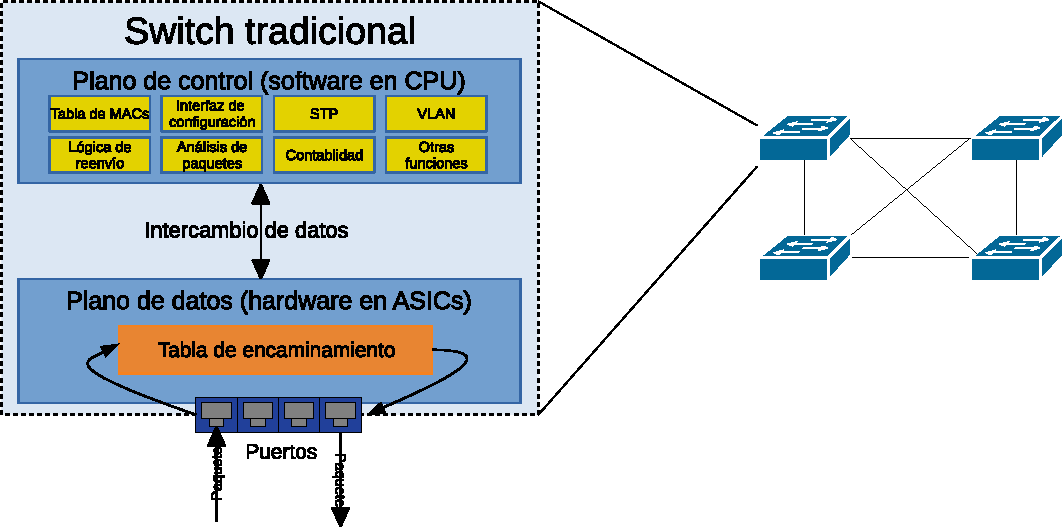
\includegraphics[width=\textwidth]{imagenes/figuras/Switch tradicional.pdf}
    \caption{Figura de planos de control y de datos}
    \label{fig:planos_red_tradicional}
\end{figure}



Como podemos ver en la figura \ref{fig:planos_red_tradicional} podemos dividir en dos planos principales a los dispositivos de red (routers y switches). Un \textbf{plano de datos} encargado de mover los paquetes que entran desde los distintos puertos siguiendo unas instrucciones (tablas de encaminamiento) y un \textbf{plano de control} encargado de calcular dichas tablas, dependiendo de las características del paquete recibido (puerto de origen, cabeceras del paquete, etc). Estos planos se encuentran dentro del mismo dispositivo y están altamente acoplados, teniendo que ser el plano de control consciente del sistema que trabaja por debajo. Normalmente el plano de datos está implementado directamente en circuitos físicos, sea mediante \acrshort{asic2}'s\footnote{Application-Specific Integrated Circuit, Circuitos hardware con una función muy específica, lo que les aporta una gran velocidad y un bajo consumo energético.} o cualquier otro tipo de hardware especializado. Este acoplamiento hace que el plano de control esté definido de forma cerrada por el fabricante del equipo y limitado a lo que el fabricante haya integrado.


El hecho de que los planos de control y de datos (y en general los equipos de red) sigan un esquema de desarrollo cerrado fijado por el fabricante hace que no se puedan actualizar las redes a los avances que la tecnología está sufriendo estos días. En los equipamientos de red esto se acentúa ya que suelen ser equipos muy caros y con una vida media de muchos años. Al final acabamos con un ecosistema de red que no puede adaptarse a las nuevas necesidades por si mismos, sino que una vez comprado e instalado es (casi) imposible actualizar la red y sus equipos y añadir nuevas funcionalidades.

Existe además una relación entre los problemas de seguridad y esta falta de flexibilidad por parte de la red. Si se descubre alguna vulnerabilidad en algún protocolo de red estamos casi seguros de que no vamos a poder mitigarlo sin tener que pagar por un equipo nuevo que incluya los parches de seguridad necesarios. Además, como el equipo de red funciona como un todo, las actualizaciones y nuevas funcionalidades tienen un ciclo de desarrollo muy lento, pues es necesario crear (o modificar) las funciones del equipo de red teniendo en cuenta todos los aspectos (software y hardware) del equipo (y en definitiva, sacar un nuevo modelo). 

Aunque se han hecho avances en la modularidad de los equipos de red (utilizando por ejemplo sistemas operativos actualizables como iOS o RouterOS) seguimos teniendo un esquema cerrado en el que los equipos de diferentes proveedores no son compatibles a la perfección entre sí.


\begin{figure}[h!]
    \centering
    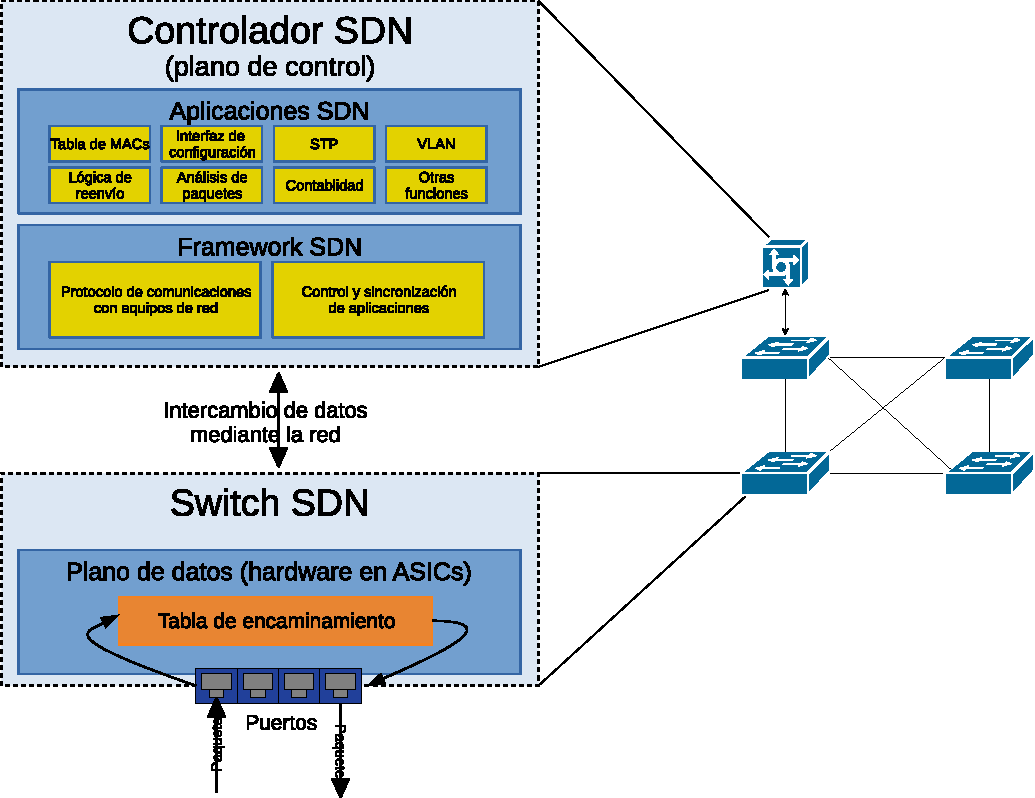
\includegraphics[width=\textwidth]{imagenes/figuras/Switch sdn.pdf}
    \caption{Figura de planos de control y de datos en SDN}
    \label{fig:planos_red_sdn}
\end{figure}

La gran revolución que presentan las Redes Definidas por Software es la separación entre el plano de control y el plano de datos de los dispositivos de la red (Figura \ref{fig:planos_red_sdn}). Hardware especializado sigue encargándose de reenviar (o no) los paquetes que llegan a los distintos puertos del dispositivo, pero es un sistema externo el que se encarga de decidir donde se tienen que enviar los paquetes (calcular las tablas de encaminamiento).

En una Red Definida por Software existe la figura del \emph{controlador de la red}, un dispositivo (normalmente un servidor) que ejecuta la lógica de la red y establece las distintas tablas y rutas que los switches tienen que seguir en el momento en el que tienen que procesar un paquete de datos. Este controlador, al ser una aplicación, puede ejecutarse en un servidor físico, una máquina virtual, agrupaciones de servidores (clusters) o incluso en servidores en la nube, proporcionando un control centralizado de lo que ocurre en la red. Además permite una comunicación del estado de la red con otras aplicaciones, lo que sirve para, si así se desea, optimizar la red en cuestión a las distintas necesidades que las aplicaciones que se ejecutan sobre ellas tengan.

Hasta ahora, la aparición de un nuevo protocolo o un nuevo problema a resolver ha conllevado iniciar un nuevo proceso de diseño de un nuevo modelo de switch o router (o sistema operativo) para implementar la solución necesaria (añadir soporte de VLAN, firewall, compatibilidad con nuevos protocolos como IPv6, etc). Mediante el enfoque de las SDN añadir nuevas funcionalidades es tan sencillo como escribir una aplicación software que resuelva el problema. Al ser un producto únicamente software este sigue su modelo de desarrollo, mucho más ágil que el desarrollo hardware y, normalmente, más barato.


\subsection{Las primeras SDNs.}

La idea de separar los planos de control y de datos apareció en 2004 mediante una propuesta de la \acrshort{ietf} publicada como RFC3746\cite{rfc3746}. Esta primera aproximación no fue bien recibida por los fabricantes de equipos de red debido a los grandes daños que podría causar un fallo en el plano de control. No fue hasta 2008 que se retomó la idea de separar los planos de control y datos de las redes de ordenadores con la propuesta de la Universidad de Stanford \cite{openflowstanford} de una \acrshort{api} \footnote{Application Programming Interface, una especificación de funciones e interfaces para que distintos programas se comuniquen entre si.} para implementar redes SDN, OpenFlow. A partir de ese momento empresas como Google \cite{hoelzlet78:online}, HP o NTT empezaron a desarrollar sus propias implementaciones de SDN, bien usando OpenFlow o diseñando sus propias APIs y protocolos. Un momento de especial interés es 2011 cuando se funda la Open Networking Fundation \cite{OpenNetw57:online}, una organización formada por operadores de red dedicada a promover las redes definidas por software y a estandarizar el protocolo OpenFlow. 

\subsection{Protocolos y estandarización.}

Aunque en este documento hemos hablado de SDN y de OpenFlow cabe destacar que no son lo mismo. SDN es un concepto de redes programables que ejecutan aplicaciones de control para gestionar el tráfico de una red. Como concepto que es se trata de una forma de diseñar redes, no de un programa específico para hacer esto. OpenFlow es un protocolo abierto de comunicación entre dispositivos de red y controladores de la misma que permiten el despliegue de redes SDN. Es, en si mismo, una especificación de una API para lograr el objetivo de crear redes definidas por software. Sin embargo existen otros protocolos (propietarios, de distintos fabricantes) que se utilizan para implementar SDN. Ejemplos de estos protocolos y arquitecturas son Cisco DNA de Cisco\cite{CiscoDNA47:online}, NETCONF (basado en XML)\cite{rfc6022} o OVSDB de OpenVSwitch \cite{OpenvSwi96:online}.

Sin embargo OpenFlow es el protocolo de comunicación con dispositivos de red para SDN más popular, debido a su carácter libre y al potente apoyo que recibe por parte de la Open Networking Foundation. Además, es soportado por una gran cantidad de fabricantes de equipos (incluso los que tienen sus propios protocolos de SDN) como Cisco, Mikrotik, HP, Jupyter Networks, etc.

El proceso de estandarización de OpenFlow está liderado por la Open Networking Foundation, que publica periodicamente nuevas versiones del protocolo, siendo la última versión la 1.5 \cite{SDNTechn21:online}. A partir de la especificación del protocolo hay diversas implementaciones del mismo (algunas propietarias) pero que son capaces de comunicarse con los dispositivos de red (hardware o virtualizados) que se adhieran al protocolo. Algunas de estas implementaciones son: OpenDayLight, RYU, NOX o Beacon \cite{ListofOp48:online}.

\subsection{Comparación con redes tradicionales: ventajas e inconvenientes.}

%Comparar facilidad de uso, despliegue, costes operativos, etc.

A continuación vamos a realizar una comparativa entre una red tradicional y una red definida por software, resaltando las posibles ventajas que puede tener una respecto a la otra dependiendo del escenario en el que nos encontremos.

Podemos empezar comentando que dependemos del escenario para elegir una arquitectura de red frente a la otra. Las SDN son por lo general más complejas que una red tradicional en escenarios donde tenemos muy pocos dispositivos, por ejemplo en una red doméstica de área local en la que no tenemos que hacer ningún tipo de ingeniería del tráfico. Sin embargo en redes corporativas donde tenemos gran cantidad de dispositivos, usuarios y requerimientos específicos nos puede ser de gran ayuda plantearnos diseñar la red con la arquitectura de SDN. Un ejemplo de esto es cuando tenemos una única infraestructura de red para ofrecer servicios diferenciados (DiffServ), en el que por una única red viajan paquetes de ordenadores, teléfonos VoIP, cámaras de seguridad, impresoras, servidores, etc. En una red tradicional podemos conseguir este tipo de red configurando manualmente cada uno de los switches y routers para poder conseguir el comportamiento esperado. Esta tarea se hace especialmente tediosa en redes muy grandes y en redes dinámicas, en las que los servicios y los requisitos cambian continuamente a medida que pasa el tiempo (empresas que se amplían, nuevos servicios, renovación de equipos, etc).

Con una red definida por software todas las tareas de administración de la red están centralizadas en el controlador y, ante la aparición de nuevos requisitos de la red, solo hay que modificar el comportamiento del mismo (o escribir uno nuevo) para poder adaptar la red a las nuevas necesidades. Además permite la integración tanto de nodos de red hardware como software, por lo que la gestión de infraestructuras virtualizadas (sea en un centro de datos propio o en la nube pública) se hace mucho más sencilla.

En una comparativa de este tipo no podemos dejar de hablar de los costes económicos de los distintos tipos de redes. Especialmente vamos a comparar los costes de capital (compra de equipos) y los costes operativos (coste de funcionamiento), también conocidos por sus siglas en inglés \acrshort{capex} y \acrshort{opex}.

\begin{itemize}
    \item CAPEX: Son los gastos de adquirir bienes en una empresa. En el contexto en el que estamos hablando ahora mismo sería el coste de los equipos y el despliegue inicial de la red. Estos son similares tanto en una red tradicional como en una red definida por software, pudiendo ser incluso menores en estas últimas. Esto se debe a que los equipos de diferentes fabricantes son compatibles entre sí, por lo que no estamos atados a un único fabricante y podemos elegir los dispositivos más competitivos económicamente.
    \item OPEX: Son los gastos de operación de una empresa. Hablando de redes son los costes derivados de mantener la red operativa y actualizada para que ofrezca el rendimiento deseado. En una red definida por software estos gastos son menores. Esto se debe a que son más fáciles de gestionar (hace falta menos personal) y a que son mucho más modulares y expandibles que las redes tradicionales. Un ejemplo de esto es que, si queremos añadir una nueva funcionalidad a la red (sin tener que adquirir nuevo equipamiento) la configuración de una red tradicional es mucho más lenta, por lo que la operación se extenderá más en el tiempo que con una SDN, con su correspondiente pérdida de dinero derivada de no tener la red al 100\% de su capacidad durante un tiempo. Además no tenemos por qué estar sometidos a los esquemas de licencias de los fabricantes de red (o al menos de un único fabricante) habiendo, al ser un mercado estandarizado e interoperable, mayor oferta de proveedores y por tanto menor coste.
\end{itemize}

Podemos resumir la comparativa entre redes tradicionales y redes definidas por software de la siguiente manera:

\begin{itemize}
    \item Ventajas de las SDN frente a las redes tradicionales:
    \begin{itemize}
        \item Gestión más sencilla.
        \item Fácilmente expandibles.
        \item No están limitadas a un único proveedor de equipos.
        \item Permiten un mayor aprovechamiento de la infraestructura existente.
        \item Reducen los costes operativos de la empresa.
        \item Aumento del rendimiento y fácil optimización.
        \item Permiten el reaprovechamiento de equipos existentes, lo que reduce costes.
    \end{itemize}
    \item Desventajas de las SDN frente a las redes tradicionales:
    \begin{itemize}
        \item Son más complejas de diseñar e implementar.
        \item Requieren una infraestructura de servidores para funcionar.
        \item No merecen la pena en redes simples.
        \item Es una tecnología en constante evolución, por lo que aún tiene mucho margen de mejora.
    \end{itemize}
\end{itemize}

En definitiva podemos ver que las redes definidas por software presentan unas ventajas nada despreciables frente a las redes tradicionales.

\section{Comparativa y elección de herramientas.}

\subsection{Sistema de emulación de redes. Laboratorio virtual}

La primera herramienta que necesitamos para desarrollar nuestro proyecto es un software capaz de emular redes de ordenadores para poder realizar todas las pruebas necesarias sobre nuestro sistema. Además, este software debe ser compatible con OpenFlow para poder implementar SDN y no una simple red tradicional. Para esto último tenemos muchas herramientas como PacketTracer de Cisco o CORE Network Emulator (entre muchos otros). Sin embargo ninguna de estas herramientas permiten emular switches compatibles con OpenFlow, por lo que no nos son de utilidad.

Revisando las opciones disponibles nos encontramos con 2 herramientas candidatas: NS3 \cite{ns3adisc22:online} y Mininet\cite{MininetA12:online}.

NS3 es un software de simulación de redes libre que permite simular redes de ordenadores en un ordenador. Mininet es un software de emulación de redes también libre que utiliza tecnologías de virtualización de Linux para generar nodos virtuales en un ordenador. En la tabla \ref{tab:mininet_ns3} vamos a comparar sus características principales.

\begin{table}[h!]
    \centering
    \begin{tabular}{|c|c|c|}
    \hline
        Característica & Mininet & NS3  \\
    \hline
         Tipo de software & Emulación & Simulación\\
    \hline
        Licencia & BSD & GPLv2 \\
    \hline
        Lenguaje & Python & C++ \\
    \hline
        Soporta OpenFlow & Si & Si \\
    \hline
        Soporta WiFi & Si & Si \\
    \hline
        Repaldado por & ONF  & Indenpendiente \\
    \hline
    \end{tabular}
    \caption{Comparativa entre Mininet y NS3}
    \label{tab:mininet_ns3}
\end{table}

Debido a su soporte por parte de la Open Networking Foundation y a que se utiliza creando scripts en python vamos a elegir \textbf{Mininet} (en su versión compatible con wifi) como software de laboratorio de pruebas para el desarrollo de nuestra red inteligente.

\subsection{Framework del controlador OpenFlow}

Como ya hemos comentado anteriormente OpenFlow es la especificación de un protocolo de comunicación entre un controlador de una SDN y el plano de datos de un switch compatible. Necesitamos elegir un framework de trabajo que nos permita escribir nuestras propias aplicaciones para la red e implemente OpenFlow para la comunicación con los switches.

En el mercado existen gran variedad de soluciones que resuelven este problema. Como estamos en un entorno académico vamos a centrarnos en las opciones que sean Open Source (código libre), pues, generalmente, presentan una mejor documentación y tienen soporte dado por una comunidad global. Al ser productos libres es muy probable que si tenemos algún problema alguien lo haya tenido ya y la solución se encuentre en internet publicada.

Entre las opciones más maduras tenemos: Ryu, OpenDayLight y POX.

En la tabla \ref{tab:comparativa_frameworks} vamos a comparar las características más reseñables de estos tres proyectos.

\begin{table}[h!]
    \centering
    \begin{tabular}{|c|c|c|c|}
    \hline
        Característica & RYU & OpenDayLight & POX  \\
    \hline
        Versión de OpenFlow & 1.5 & 1.3 & 1.0 \\
    \hline
        Licencia & Apache & Eclipse & Apache \\
    \hline
        Lenguaje & Python 3 & Java  & Python 2\\
    \hline
        Documentación disponible & Bastante & Mucha  & Suficiente \\
    \hline
        Último commit a su repositorio & 2020 & 2020  & 2017 \\
    \hline
        Desarrollado por & FaucetSDN  & Linux Foundation  & Nicira Inc.\\
    \hline
    \end{tabular}
    \caption{Comparativa entre frameworks OpenFlow}
    \label{tab:comparativa_frameworks}
\end{table}

Por su soporte de OpenFlow, su documentación y estar programado en Python utilizaremos \textbf{Ryu} como framework de desarrollo del controlador de nuestra SDN.

\subsection{Otras herramientas}

Además del laboratorio de pruebas y el framework de OpenFlow necesitaremos algunas herramientas adicionales para poder diseñar, implementar y probar nuestra red. Primeramente necesitaremos un software de análisis de tráfico que nos ayude a ver el camino que los paquetes siguen en nuestra red. La herramienta \emph{de facto} en el desarrollo de redes bajo el sistema operativo Linux es \textbf{Wireshark}, que nos permite capturar y analizar paquetes desde cualquier interfaz a la que tengamos acceso. Mininet nos proporciona interfaces virtuales que nos permiten escuchar cada uno de los enlaces que estamos virtualizando.

También nos hace falta alguna manera de generar tráfico en nuestra red para así poder estimar su rendimiento. Para esto vamos a utilizar dos herramientas diferentes. Por un lado tenemos \textbf{iperf}, que nos permite generar un flujo de paquetes controlando el ancho de banda que queremos consumir (o generando todo el tráfico que pueda y así probar a sobrecargar los enlaces y con ello, finalmente, la red). Utilizaremos adicionalmente el generador de tráfico \textbf{D-ITG}, una herramienta que nos permite simular distintos patrones de tráfico como VoIP, juegos online, tráfico HTTP, etc. Lo que nos permitirá mejorar nuestra capacidad de análisis sobre el rendimiento de la red haciendo una simulación de carga de trabajo que se ajuste mejor a los requisitos.


%\chapter{Pruebas de herramientas: red sencilla}
%MOVER ESTE CAPITULO A OTRA PARTE (SI LLEGA A HACERSE).
%Una simple topo linear de mininet con un controlador de ryu.

%\section{Comparativa con redes convencionales.}


\chapter{Planificación y estimación de costes.}

\section{Temporización}

\begin{table}[!h]
\centering
\begin{tabular}{|l|l|l|}
\hline
Nombre & Fecha de inicio & Fecha de fin \\ \hline
Planteamiento de la propuesta & 3/2/20 & 28/2/20 \\ \hline
Investigación sobre SDN & 2/3/20 & 29/5/20 \\ \hline
Desarrollo de la memoria & 16/6/20 & 8/9/20 \\ \hline
Diseño de la red & 1/6/20 & 8/6/20 \\ \hline
Pruebas con Ryu & 22/6/20 & 9/7/20 \\ \hline
Implementación del controlador & 20/7/20 & 2/9/20 \\ \hline
Evaluación de la red & 3/9/20 & 7/9/20 \\ \hline
\end{tabular}
\label{tab:temporizacion}
\caption{Temporización del proyecto}
\end{table}

Este proyecto se ha planificado siguiendo la temporización que se detalla en la tabla \ref{tab:temporizacion}, contando con periodos vacacionales.

Reflejado en un diagrama de Gantt la temporización ha sido la siguiente:

\begin{figure}[!h]
    \centering
    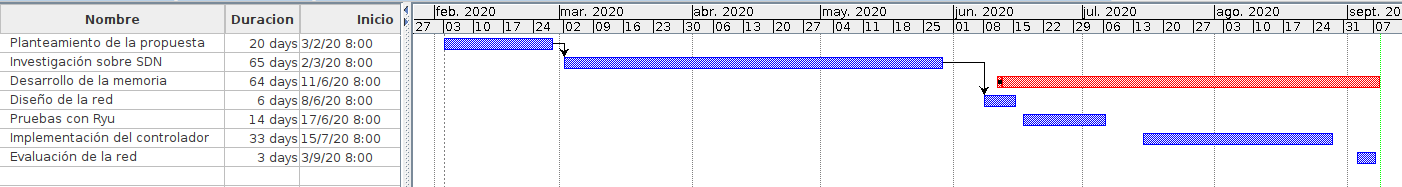
\includegraphics[width=1.2\textwidth]{imagenes/figuras/temporizacion.png}
    \caption{Diagrama de Gantt del proyecto}
    \label{fig:temporizacion}
\end{figure}

\section{Presupuesto}

Si tuviéramos que implementar este proyecto en un entorno físico tendríamos una serie de gastos que vamos a reflejar a continuación. En este presupuesto no se incluyen los nodos cliente de la red ni el cableado, solo lo necesario para que la red definida por software funcione correctamente. Vamos a optar por switches de la marca Mikrotik por su compatibilidad con OpenFlow y su bajo precio. Para ejecutar el controlador Ryu y el servidor DHCP vamos a utilizar un sistema basado en una Raspberry Pi 4, que ofrece suficiente capacidad de computación para la tarea a desempeñar.

El presupuesto queda de la siguiente manera:

\begin{figure}[!h]
\centering
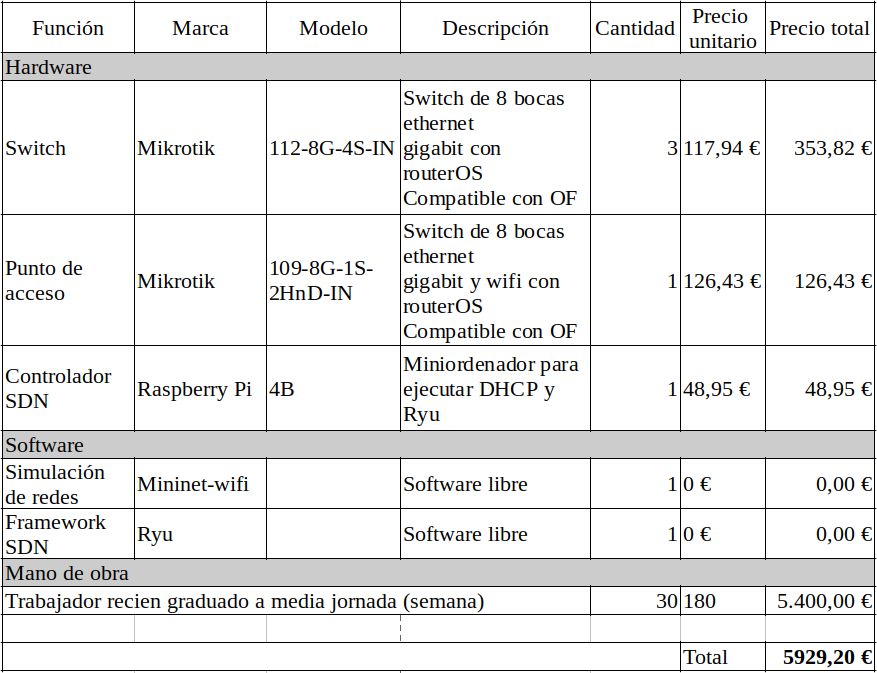
\includegraphics[width=\textwidth]{imagenes/figuras/presupuesto.png}
\label{tab:presupuesto}
\caption{Presupuesto del proyecto}
\end{figure}

La diferencia con un presupuesto con una red tradicional (no SDN) es la Raspberry Pi. Si comparamos su precio con el ahorro que supone la configuración automática de nuevos nodos en materia de gastos de personal y de tiempo de mantenimiento de la red podemos afirmar que merece la pena estructurar la red como una Red Definida por Software. El precio de la mano de obra se ha calculado como 30 semanas de trabajo a media jornada teniendo en cuenta los salarios medios de los ingenieros informáticos recién graduados \cite{Cuantoco58:online}
%
\chapter{Diseño de la propuesta}

En este capítulo vamos a analizar los requisitos de nuestra red y a establecer una propuesta de diseño físico para la misma. Además vamos a caracterizar los distintos nodos que compondrán nuestra red.

Vamos a partir del plano de nuestra oficina en la que queremos montar la red. Como aproximación vamos a suponer que se trata de una nueva oficina de la Universidad de Granada en la que van a encontrarse 5 trabajadores, cada uno de ellos con sus respectivos puestos de trabajo. La planta de la oficina sería la mostrada en la figura \ref{fig:planta_oficina}:

\begin{figure}[!h]
    \centering
    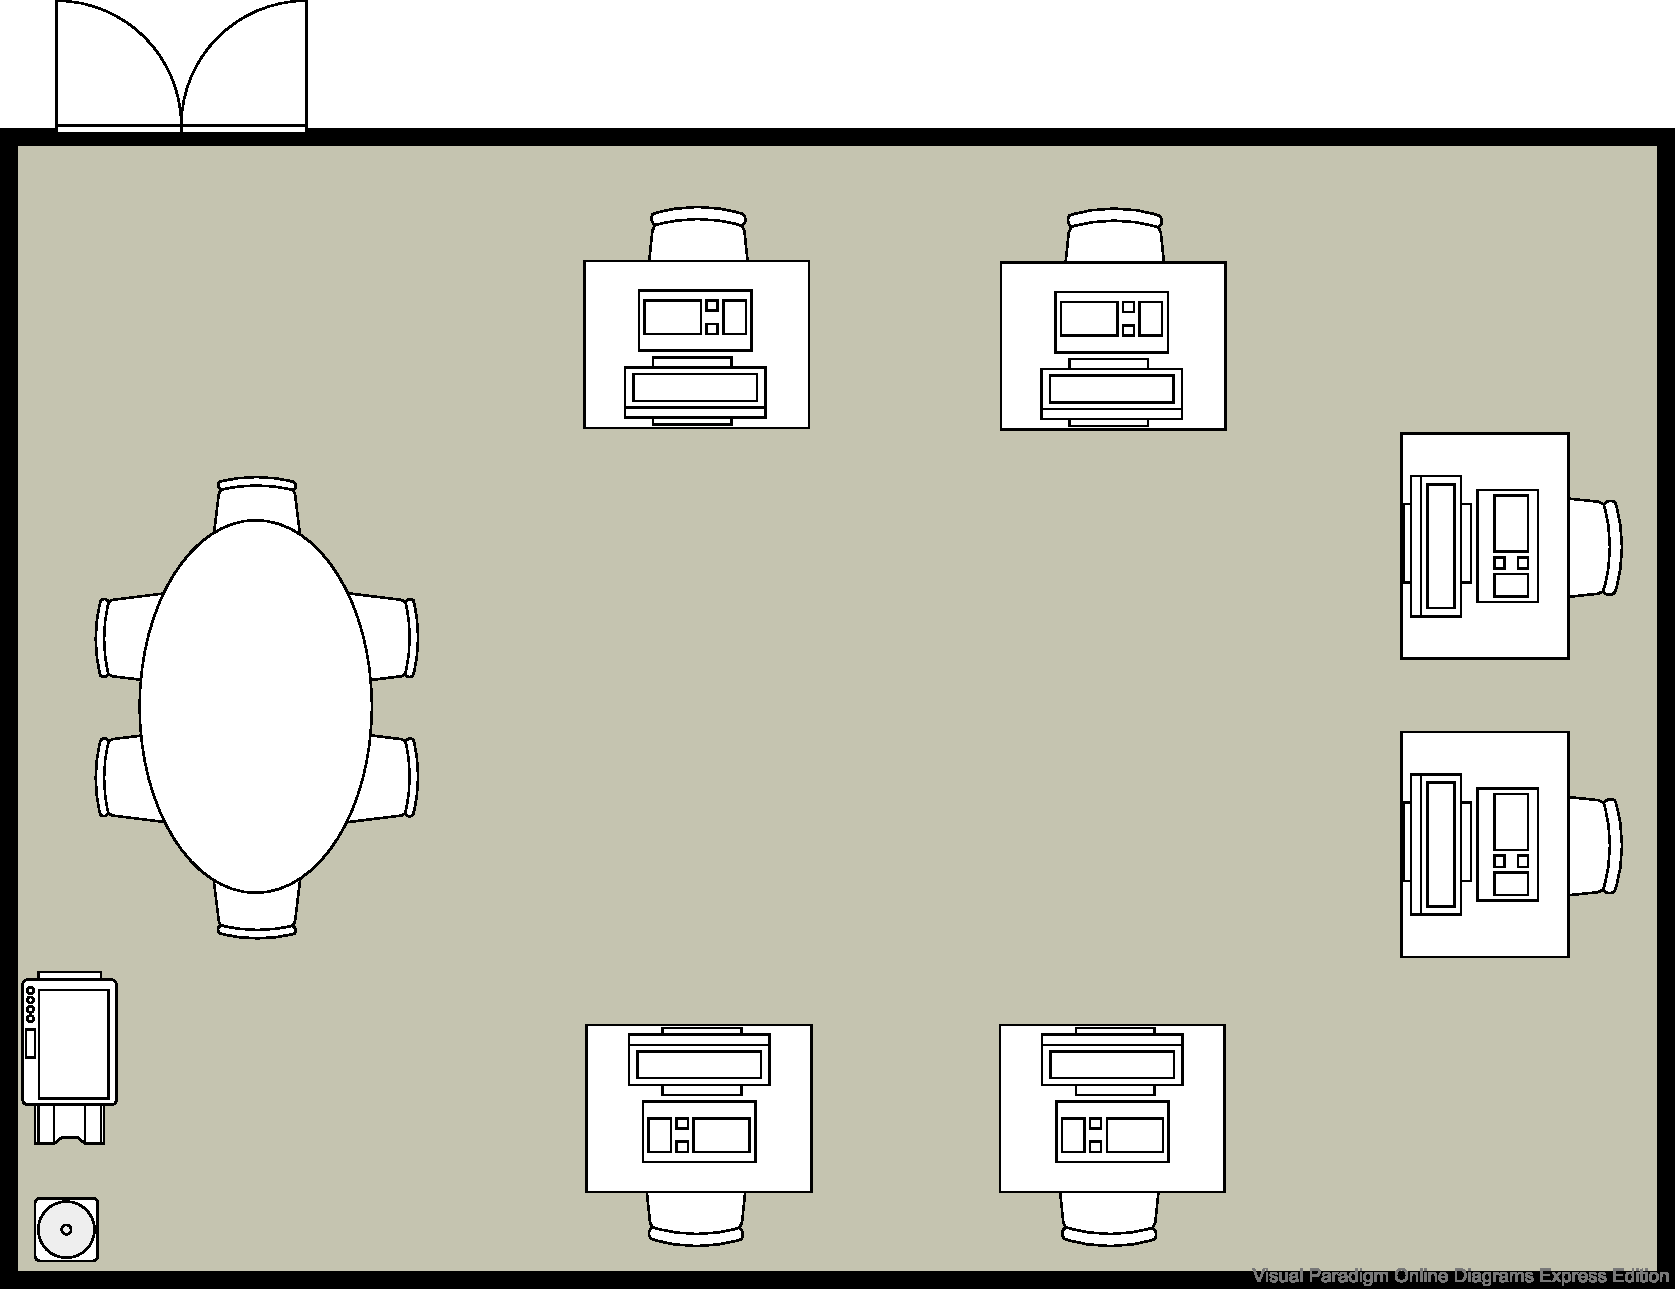
\includegraphics[width=\textwidth]{imagenes/figuras/Plano oficina.pdf}
    \caption{Planta de la oficina en la que vamos a montar nuestra red.}
    \label{fig:planta_oficina}
\end{figure}

A partir de este plano vamos a identificar los requisitos que debe cumplir nuestra red y vamos a hacer un diseño base para la misma. Además veremos como no tenemos que decidir exactamente cuantos equipos finales habrá en la misma ni a donde van conectados, pues la red será capaz de detectarlos automáticamente y configurarlos según su tipo.

\section{Requisitos de una red corporativa}

Empezaremos describiendo el entorno en el que nos encontramos y obteniendo los distintos requisitos funcionales de la red, para luego identificar los tipos de nodo que se han de conectar así como las tareas que deben desempeñar los usuarios finales para utilizar nuestra red.

\subsection{Descripción del entorno y análisis de requisitos}

En esta propuesta nos encontramos en una oficina con puestos informáticos, teléfonos VoIP y una impresora compartida. Además sabemos que se quiere instalar una red de videovigilancia en la oficina para controlar la seguridad. Queremos diseñar una red que sea eficiente en rendimiento y coste a la vez que sea segura y, automáticamente se pueda ampliar tanto como se necesite (así como instalar redes similares en múltiples oficinas).

Formalmente la lista de requisitos funcionales de la red es la siguiente:

\begin{itemize}
    \item La red debe estar operativa las 24 horas del día, 7 días a la semana (24x7).
    \item Solo se instalará un único cableado para los distintos dispositivos, es decir, la las mismas líneas de datos transportarán datos de las cámaras de seguridad, los teléfonos, los ordenadores y cualquier otro dispositivo que se pueda (quiera) conectar.
    \item Se incluirá acceso mediante red WiFi para los dispositivos de los trabajadores y los posibles clientes.
    \item Deberá poderse ampliar la red sin tener que instalar una nueva, simplemente añadiendo los dispositivos necesarios sin tener que tocar ninguno de los existentes.
    \item Los usuarios no son expertos en tecnologías, por lo que debe una ser red fiable que no les ocasione molestias a la hora de trabajar.
    \item La red se debe poder administrar remotamente, para evitar desplazamientos de técnicos a la oficina.
    \item Los usuarios no deben poder conectarse a la red de seguridad desde sus dispositivos (ordenadores de trabajo o dispositivos WiFi). Si deben poder conectarse entre ellos y al servidor de contenido sobre el que trabajan.
    \item Los usuarios podrán utilizar recursos compartidos como la impresora de red.
    \item La red deberá ser tolerante a fallos.
\end{itemize}

Ahora vamos a caracterizar los distintos elementos que conforman nuestra red antes de hacer el diseño.

\subsection{Tipos de nodos}

A nuestra red deberán conectarse: ordenadores de los trabajadores (puestos fijos), teléfonos VoIP, cámaras de seguridad, impresoras en red y dispositivos inalámbricos. Cada uno de los tipos de nodos tienen unos requisitos distintos: de esta forma los teléfonos tienen la necesidad de enviar y recibir paquetes con la menor latencia posible (aunque permiten que se pierdan algunos paquetes); las cámaras de seguridad admiten paquetes con latencia alta y pérdida de paquetes, pero tienen un requisito de ancho de banda constante al estar continuamente enviando vídeo al servidor de seguridad para su grabación. Los ordenadores y la impresora no tienen requisitos de velocidad (siempre que ofrezcan un rendimiento suficiente que no empeore la calidad de la experiencia de los trabajadores, es decir, que no sea tan lenta que los usuarios desesperen) pero admiten que se pierdan paquetes de datos.

\subsection{Usuarios finales}

Los usuarios finales de la red son los trabajadores de la oficina y los clientes o colaboradores que traigan sus propios dispositivos y necesiten una conexión de red. Estos usuarios no deben tener consciencia de la red desde un punto de vista técnico. Su mayor relación con la red será introducir la clave de acceso a la red inalámbrica en sus dispositivos, nada más.

\subsection{Tareas de administración}

Las tareas de administración sobre la red tendrán que ser mínimas, siendo la principal el cambio de la clave de acceso de la red inalámbrica. Cuando sea necesario instalar un nuevo dispositivo, el administrador solo deberá encargarse de conectarlo a la red, y esta última será la encargada de configurar de forma automática todos los parámetros del nuevo dispositivo (Dirección IP, puerto de acceso, permisos de acceso a otros dispositivos, etc.).

\section{Diseño físico de la red.}

Vamos a realizar el planteamiento físico de la red sobre el plano de planta de la oficina expuesto anteriormente. En la figura \ref{fig:diseño_fisico} vemos como queda planteado el diseño física. Ahora vamos a discutir algunas cuestiones de diseño para entender como llegamos hasta él.

En primer lugar está la decisión de cuantos switches poner, en este caso hemos optado por 3 switches ethernet y un punto de acceso inalámbrico. Otra opción sería poner un único switch grande pero por razones de costo (un switch grande compatible con OpenFlow es mucho más caro que varios más pequeños también compatibles) se ha decidido la opción de múltiples switches. Luego está la topología a usar. Cisco recomienda en sus diseños utilizar topologías en árbol, donde los switches de acceso (a los que se conectan los usuarios finales) se conectan entre sí a otros swiches de niveles superiores \cite{cisco:10.5555/975411}. Sin embargo nosotros hemos elegido empezar con una topología en malla donde los switches están interconectados entre sí. Esta configuración nos permite tener una mayor redundancia en caso de caída de enlaces y nos permitirá, en caso que sea necesario, ejecutar aplicaciones de enlaces redundantes en el controlador SDN si necesitáramos mayor ancho de banda en la red, sin tener que cambiar las conexiones existentes. Esta topología nos permite ampliar la red de forma sencilla asegurando la redundancia. La topología en malla introduce un problema que tendremos que resolver: la aparición de bucles en la red. Estos bucles pueden ser eliminados de la topología lógica de la red utilizando el protocolo \acrshort{stp}, \acrlong{stp}, que detecta los bucles en la red y deshabilita los puertos que lo causan, volviéndolos a activar en caso que sean necesarios (caída, sobrecarga, agrupamiento de enlaces, etc). Además podemos ver que en nuestro diseño no existen capas diferenciadas entre switches de acceso y de distribución, sino que todos los switches son de acceso (donde se conectan los usuarios finales). De este modo no estamos introduciendo en la red más dispositivos que mantener y que, principalmente, comprar.

\begin{figure}[!h]
    \centering
    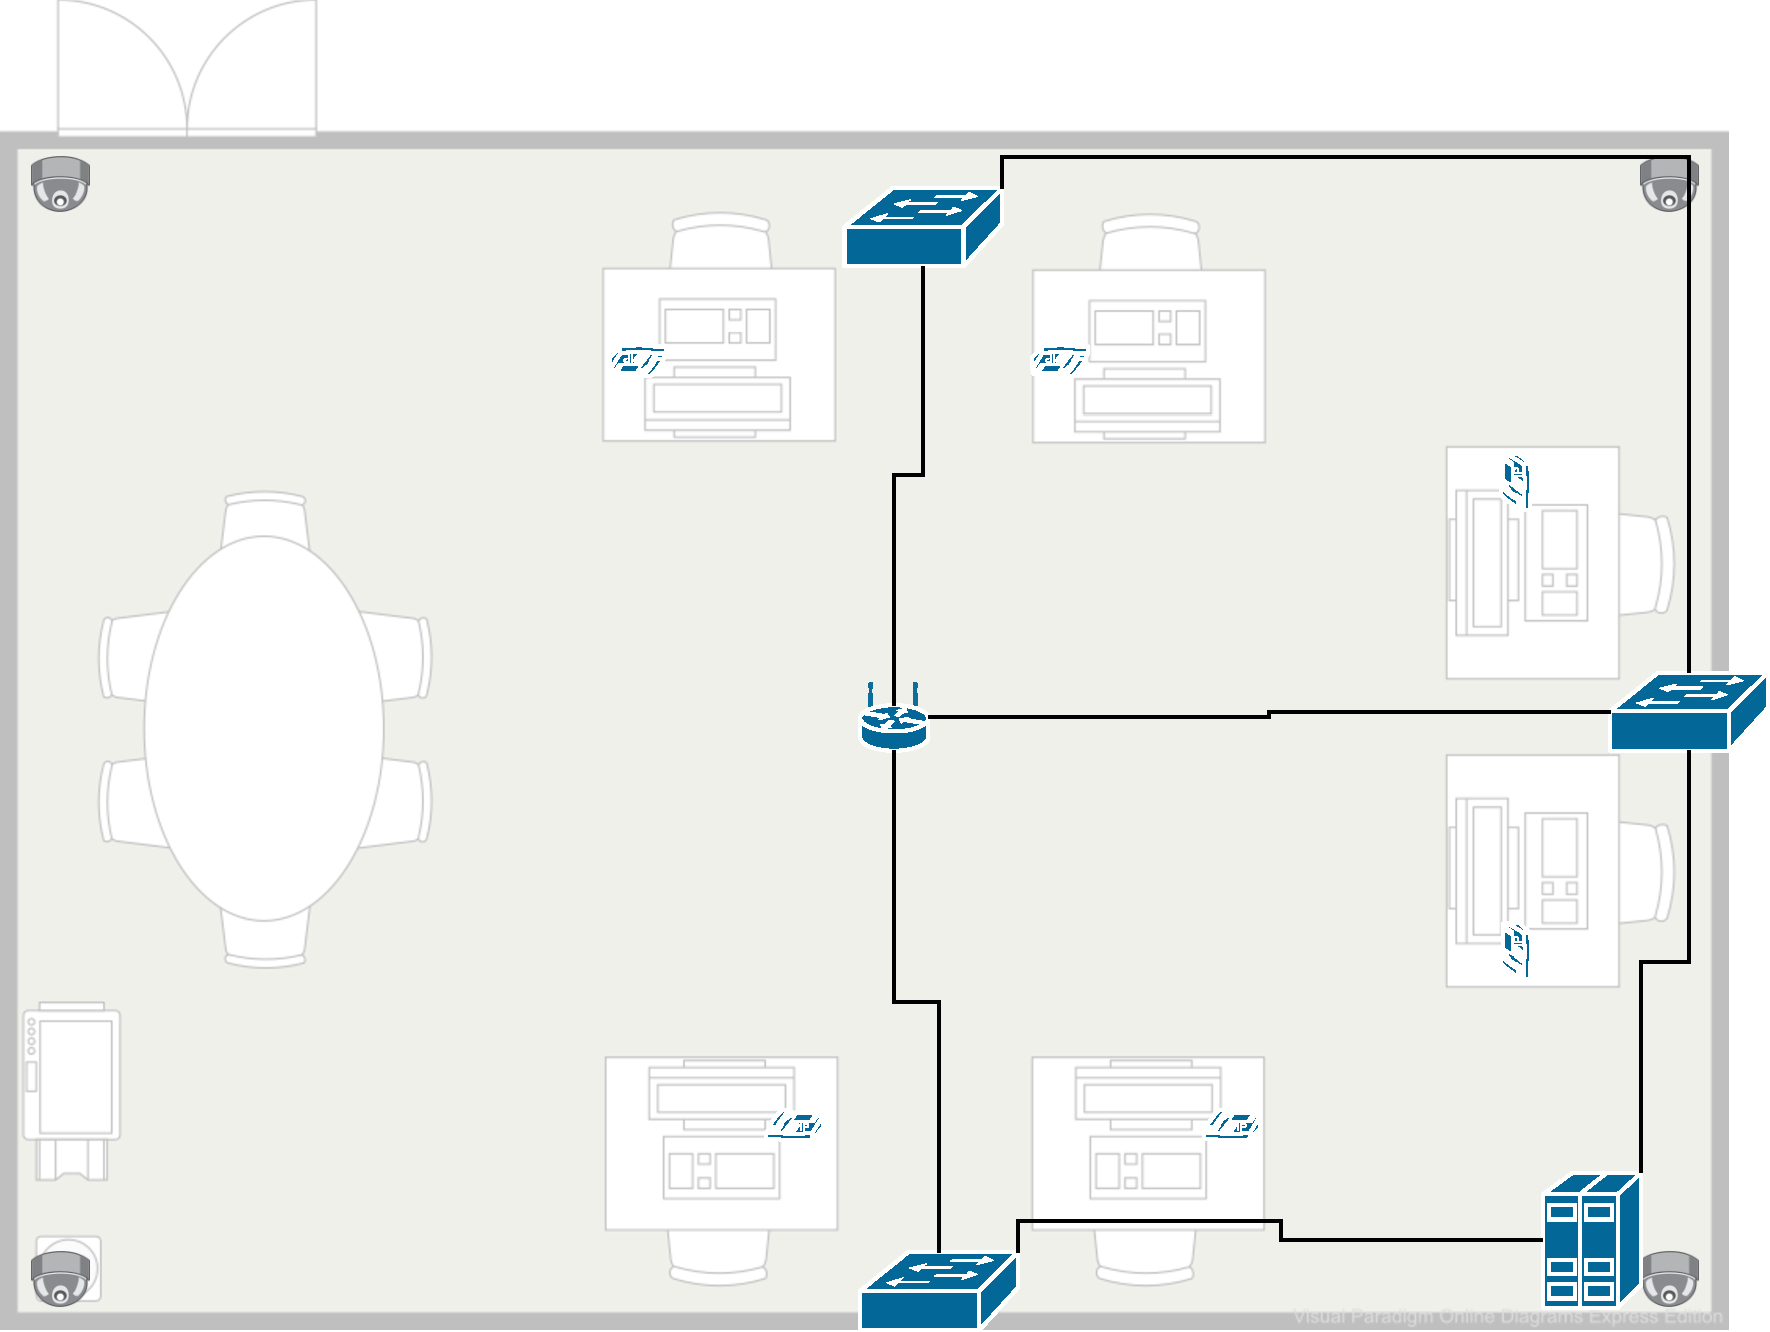
\includegraphics[width=\textwidth]{imagenes/figuras/requisitos_red_con_plano.pdf}
    \caption{Diseño físico de la red.}
    \label{fig:diseño_fisico}
\end{figure}

\section{Diseño lógico de la red.}

Una vez tenemos el diseño físico de la red (los dispositivos propiamente dichos) vamos a encargarnos del diseño lógico, es decir, como tiene que estar configurada la red para funcionar correctamente y cumplir los requisitos que hemos identificado anteriormente.

Un punto vital a tener en cuenta en este apartado es que estamos diseñando una red definida por software, con todas las ventajas que ello conlleva, por lo que tenemos que pensar en como solucionar los problemas de una forma abstracta y general, pues el controlador (la aplicación que genera las tablas de encaminamiento de los switches) es el mismo para todos los switches de la red, por lo que tendremos que pensar en la red completa como un todo y no pensar cosas como \emph{''Pues este switch que está cerca de la impresora lo configuro de una manera y el de la otra esquina de la sala, de otra manera completamente diferente''} ya que esa forma de diseñar redes conlleva problemas de mantenimiento (configuración separada de cada dispositivo de red) y no estaríamos aprovechando la capacidad que nos brindan las SDN de tratar la red como un proyecto software que podemos modificar y optimizar de forma incremental para resolver los problemas que nos puedan surgir. Recordemos que en una red tradicional una vez compras un equipo específico no nos podemos salir de las características que trae de fábrica, en una SDN podemos instalar y ejecutar tantas funcionalidades como aplicaciones desarrollemos.

Tenemos que separar los dispositivos en distintas subredes, de forma que diferenciemos los distintos servicios y no puedan verse entre ellos. Si solo hiciéramos esta distinción usando distintas redes IP los dispositivos podrían seguir comunicándose si así se quisiera (posible ataque a la red) ya que seguirían conectados a la misma red ethernet de área local (aunque sus direcciones IP no estuvieran en la misma subred). Por esto vamos a dividir la red en 3 \acrshort{vlan}\footnote{\acrlong{vlan}, redes LAN que funcionan en una misma infraestructura de red pero que lógicamente, son independientes entre si} distintas: Seguridad, telefonía y acceso general. Para lograr esta separación tenemos que encontrar alguna manera de asignar a cada dispositivo una VLAN distinta de forma automática, para mantener así la característica autoconfigurable de la red. Esta es una tarea que podemos lograr fácilmente mediante una aplicación de Ryu que asigne a cada puerto de cada switch una VLAN distinta.

Además necesitamos disponer de uno o varios servidores que ejecuten los servicios necesarios (ruteo de paquetes hacia internet, servidor de videovigilancia, servidor de telefonía e incluso el propio controlador de la red, entre otros servicios que pueden surgir más adelante). Este servidor tiene que ser accesible por todos los dispositivos, por lo que tendrá (o tendrán) que ser parte de todas las VLAN. 

Con esta información podemos generar un esquema lógico de la red que estamos diseñando. Este esquema es la figura \ref{fig:diseño_logico}.

\begin{figure}[!h]
    \centering
    \includegraphics[width=\textwidth]{imagenes/figuras/diseño_logico.pdf}
    \caption{Diseño lógico de la red.}
    \label{fig:diseño_logico}
\end{figure}

Aquí podemos ver las distintas VLAN y como están interconectados los distintos equipos de la red. En color rojo tenemos los enlaces pertenecientes a la VLAN de acceso general, en verde tenemos los enlaces de la VLAN de seguridad y en azul tenemos los enlaces pertenecientes a la red virtual de telefonía. Además en negro tenemos los enlaces \emph{trunk}, es decir, los enlaces que llevan paquetes de múltiples VLANs.


\section{Implementación de la red en un entorno virtualizado}

Una vez que hemos analizado los requisitos de nuestra red y terminado el diseño lógico de la red podemos simular dicho escenario en un laboratorio de pruebas virtual para poder hacer pruebas 

\subsection{Diseño general en MiniEdit}
Vamos a empezar haciendo un esquema básico de la red utilizando el editor gráfico de Mininet: MiniEdit

Cabe destacar que, debido a capacidad limitada de procesamiento vamos a limitar la maqueta de la red a solo dos dispositivos de cada tipo. Como podemos ver en la Figura \ref{fig:miniedit} MiniEdit nos permite crear un armazón de la red que luego podremos modificar libremente. Esto es debido a que MiniEdit permite exportar un script Python que ejecuta la red. Este script puede ser modificado para ajustar parámetros de los nodos de red que no están disponibles desde la interfaz gráfica.

\begin{figure}[!h]
    \centering
    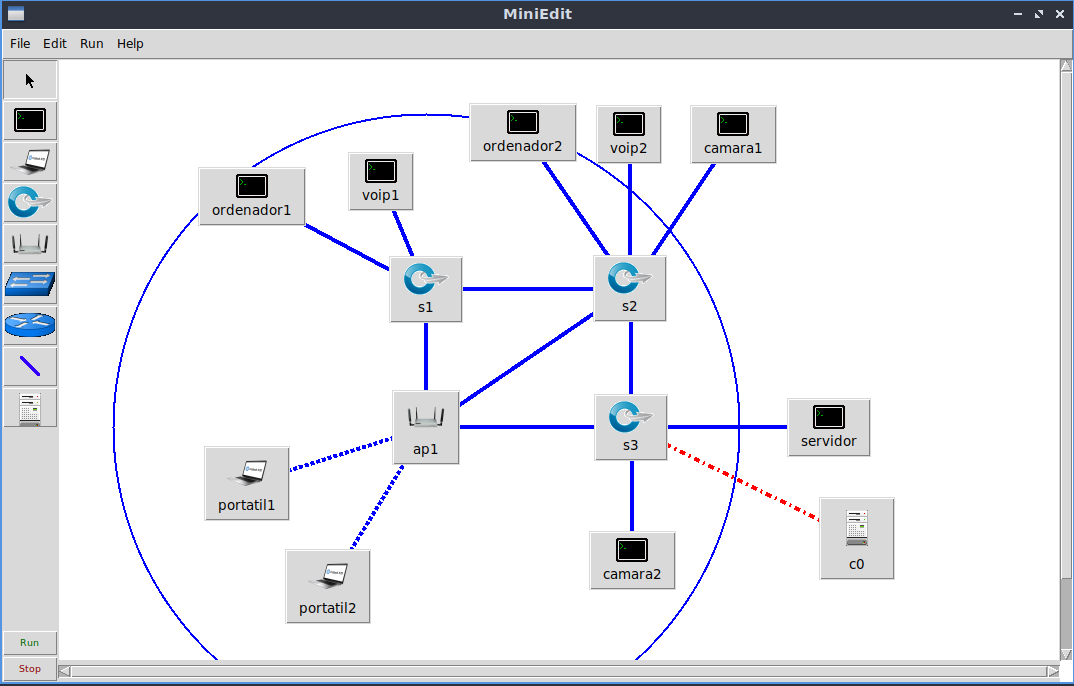
\includegraphics[width=\textwidth]{imagenes/figuras/miniedit.png}
    \caption{Maqueta de la red en la interfaz gráfica de MiniEdit}
    \label{fig:miniedit}
\end{figure}

Ahora podemos exportar el mapa a un archivo ejecutable en una consola para simular nuestra red.

Haciendo unos retoques al archivo exportado tenemos nuestra topología \footnote{Archivo topologia\_oficina.py}, que podemos ejecutar mediante

\lstinline{sudo python topologia_oficina.py}

\subsection{Caracterización de nodos}
En este apartado vamos a caracterizar los tráficos de cada uno de los dispositivos de red, para luego poder simularlos con D-ITG y poder hacer pruebas sobre la capacidad de la red.

\subsubsection{Puestos de trabajo finales}
Los puestos de trabajo están formados por un ordenador de sobremesa. Estos realizarán tareas de compartición de archivos con un servidor central y navegación puntual por internet. No tienen grandes requerimientos de ancho de banda pero si de disponibilidad, para evitar caídas del servicio, sobre todo en horario laboral.

En nuestro entorno de pruebas vamos a utilizar un perfil del generador de tráfico que mantenga un tráfico constante de baja velocidad con picos de hasta 4 Mbps. Este lo hemos extraído de la documentación oficial de la herramienta.\cite{DITG281M63:online}

\lstinline{ITGSend -a <ip_receptor> -T TCP -B E 100 W 4 1000 -o 600}

\subsubsection{Teléfonos IP}
Junto a los ordenadores de sobremesa se encuentra un teléfono IP. Estos están conectados a una red separada de los ordenadores y tienen un bajo requerimiento de ancho de banda pero si son muy sensibles a latencia y jitter en la red, por lo que la red debería ser capaz de proveer algún mecanismo de calidad de servicio para evitar bajadas de calidad en la comunicación.

El generador de tráfico tiene un mecanismo integrado de generación de tráfico que simula una conversación VoIP.

\lstinline{ITGSend -a <ip_receptor> VoIP}

\subsubsection{Dispositivos auxiliares: impresoras en red}
Además se va a instalar una impresora compartida entre todos los ordenadores de la red. Su único requerimiento es estar disponible a los usuarios cuando estos quieran utilizarla.

A la impresora simplemente le vamos a realizar pings, puesto que su carga de red no es significativa en el entorno que estamos estudiando.

\subsubsection{Cámaras de videovigilancia}
En el escenario que estamos planteando se va a incluir una red de videovigilancia. Las cámaras IP habituales tienen unos requisitos medios de ancho de banda ya que envían la señal comprimida al servidor central. Los flujos de vídeo además toleran bien la pérdida de paquetes siempre que esta no sea muy significativa. \cite{boulos:hal-00354947}. Lo realmente importante en este punto es que las cámaras no sean accesibles por ningún otro dispositivo de la red que no sea parte de la subred de seguridad.

Basándonos en una instalación preexistente de seguridad con una cámara IP con una resolución de 1280x720 píxeles hemos determinado que un ancho de banda constante de 70Kbps son suficientes para enviar vídeo al servidor de seguridad. Por esto el tráfico generado será el siguiente:

\lstinline{ITGSend -a <ip_receptor> -T UDP -C 100 -c 70}

\subsubsection{Red wifi: móviles y portátiles}

En el escenario que estamos planteando necesitamos que la red wifi sirva de acceso a los mismos recursos que los ordenadores de sobremesa, puesto que los empleados tienen sus propios dispositivos portátiles de trabajo y deberían ser capaces de usarlos en la oficina. Sus requisitos son exactamente los mismos que los puestos fijos de trabajo.


%
\chapter{Implementación y despliegue de la red.}

En este capítulo se expone el proceso de implementación de la red para cumplir los requisitos expuestos anteriormente. Empezamos generando un archivo de topología correcto a partir del esquema generado por MiniEdit para llegar a tener una simulación realista de la red, en la que los nodos no están configurados y tienen que obtener su propia configuración por parte de la red. Después implementamos la lógica de red para permitir la configuración dinámica de la misma sin necesidad de actuaciones manuales por parte de un operador. Finalmente exponemos como desplegar un entorno de pruebas para evaluar las prestaciones de la red.

En resumen, los pasos a seguir para implementar la red son:

\begin{itemize}
    \item Generar el archivo de topología final
    \item Preparar el servidor DHCP
    \item Activar el protocolo STP para evitar bucles.
    \item Activar el descubrimiento de topología de la red para distinguir enlaces trunk y de acceso
    \item Implementar el reenvío de paquetes condicionado por VLANs.
\end{itemize}


%\todo{quizás se podría llamar: diseño y despliegue de la rd? No suena bien desarrollo, en este contexto. DONE. ¿Aquí capturas de código entero o solo las partes relevantes?}
\section{Despliegue de la red en Mininet}

El archivo generado por MiniEdit contiene una serie de parámetros de configuración que no deseamos tener. Estos son, principalmente la asignación de direcciones IP a los nodos de la red. Como nuestro objetivo es que la red sea autoconfigurable tenemos que eliminar dichos parámetros. Además, ya que la identificación de nodos está basada en su dirección MAC tenemos que ajustar dichas direcciones a unos valores conocidos de antemano. Esto es así ya que si no damos ningún valor a las direcciones MAC estas se generan de forma aleatoria al arrancar Mininet, lo que hace que solo tengamos nodos en una VLAN (la VLAN por defecto).

Por esto hacemos los siguientes cambios a la configuración de los nodos:

\begin{lstlisting}[language=python, label=lst:miniedit-host, caption={Determinación de las direcciones MAC en los hosts Mininet}]
# h1 = net.addHost('h1', cls=Host, ip='10.0.0.2/24')
# h2 = net.addHost('h2', cls=Host, ip='10.0.0.3/24')
# ...

h1 = net.addHost('h1', cls=Host, ip=None, mac='00:00:00:00:00:01')
h2 = net.addHost('h2', cls=Host, ip=None, mac='00:00:00:00:00:02')
# ...

\end{lstlisting}

Así mismo tenemos que activar el soporte de la versión 1.3 del protocolo OpenFlow, ya que por defecto solo está activa la versión 1.0.

\begin{lstlisting}[language=python, label=lst:miniedit-switch, caption={Activación del protocolo OF1.3 en switch Mininet}]
s1 = net.addSwitch('s1', cls=OVSKernelSwitch, protocols="OpenFlow13")
\end{lstlisting}

Una vez arrancamos la red por primera vez y hacemos una captura de tráfico inicial comprobamos que está siendo inundada por paquetes de tipo ICMPv6 relacionados con el protocolo SLAAC de autoconfiguración de IPv6 \cite{rfc4862}. Como no estamos interesados en la configuración de IPv6 en nuestra red vamos a desactivar el protocolo en todos los nodos de la red. Para ello añadimos las siguientes líneas a nuestro script.

\begin{lstlisting}[language=python, label=lst:miniedit-ipv6, caption={Desactivación de IPv6 en nodos Mininet (Linux)}]
    info( '*** Desactivar IPv6\n')
    for h in net.hosts:
        h.cmd("sysctl -w net.ipv6.conf.all.disable_ipv6=1")
        h.cmd("sysctl -w net.ipv6.conf.default.disable_ipv6=1")
        h.cmd("sysctl -w net.ipv6.conf.lo.disable_ipv6=1")
\end{lstlisting}

Además tenemos que activar el protocolo DHCP, tanto en los clientes como en el servidor para poder proporcionar configuración automática de los equipos. Para esto añadimos al final del fichero de topología las siguientes líneas:

\begin{lstlisting}[language=python, label=lst:miniedit-dhcp, caption={Activación del servidor y clientes DHCP al arranque de la red.}]
info( '*** Iniciando el servidor DHCP \n')
    router.cmd("systemctl stop isc-dhcp-server")
    router.cmd("rm /var/lib/dhcp/dhcpd.leases")
    router.cmd("rm /var/lib/dhcp/dhcpd.leases~")
    router.cmd("touch /var/lib/dhcp/dhcpd.leases")
    router.cmd("dhcpd -4 -f --no-pid &")
    
    info( '*** Habilitando DHCP en los hosts\n')
    for h in net.hosts:
    	if h != router:
        	h.cmd("dhclient &")
\end{lstlisting}

Con estos cambios introducidos en el fichero de topología ya tenemos un conjunto de redes interconectados entre sí que simula el escenario propuesto por este trabajo y sobre el que ya podemos empezar a hacer pruebas del controlador SDN.


\section{Infraestructura de Ryu}

Ryu es un framework SDN escrito en Python basado en una estructura de aplicaciones independientes que se comunican entre sí mediante un bucle de eventos. Por esto es capaz de encadenar varias funcionalidades en un único controlador. Nuestra misión es escribir una aplicación Ryu que gestione diversos eventos relacionados con la red, siendo el principal evento a implementar el de la lógica de reenvío de paquetes. El controlador Ryu está encargado de determinar hacia donde se reenvían los paquetes que llegan a los distintos switches de la red y, si es necesario, de instalar las rutas en la tabla de rutas del switch para evitar que los paquetes sean enviados al controlador. Podemos ver un ejemplo básico de lógica de reenvío en la figura \ref{fig:primerpaquete}

\begin{figure}[!h]
    \centering
    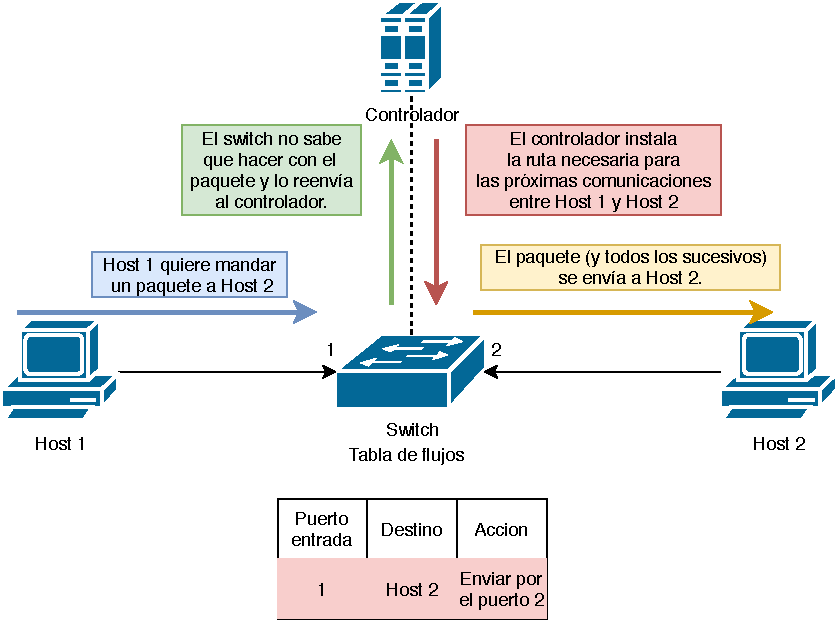
\includegraphics[width=\textwidth]{imagenes/figuras/primerpaquete.pdf}
    \caption{Ejemplo de instalación de ruta en la tabla de flujos de un switch OpenFlow}
    \label{fig:primerpaquete}
\end{figure}

En el flujo de control del controlador trabajamos únicamente respondiendo a eventos o mensajes de cualquiera de los switches o aplicación Ryu de una forma análoga a como lo hace un servidor web respondiendo peticiones de los usuarios. Para lograr una persistencia de datos y poder tomar decisiones sobre la red necesitamos persistencia de datos entre eventos en el controlador. Esto es fácilmente alcanzable mediante el uso de clases y objetos Python. Partimos de la base de que una aplicación Ryu es una clase en la que podemos guardar, por ejemplo, una descripción de la red o la tabla de direcciones MAC que conocemos.

Ahora vamos a describir las funcionalidades que hemos implementado en nuestro controlador Ryu: Switching, VLANs dinámicas, descubrimiento de topología y protocolo STP.

\subsection{Aplicación switch}

La base de todo switch es reenviar paquetes que entran al switch al nodo adecuado, evitando en la medida de lo posible enviar paquetes a nodos que no son el receptor. Con los switches tradicionales tenemos un hardware encargado de analizar los paquetes y reenviarlos al puerto adecuado de forma automática. Cuando estamos trabajando con switches SDN toda la funcionalidad tiene que ser implementada en el controlador. Esto tiene tanto ventajas (podemos configurar el reenvío como queramos) como desventajas (si nos olvidamos de alguna funcionalidad esta no estará disponible de forma automática).

Como punto de partida para nuestra aplicación hacemos una lectura de la aplicación integrada en Ryu llamada simple\_switch\_13.py. En esta aplicación se indica como programar un controlador SDN para implementar la funcionalidad básica de un switch tradicional (reenvío de paquetes con aprendizaje de direcciones MAC). A partir de este esquema podemos empezar a trabajar en nuestro propio controlador.

Una de las partes más relevantes es la primera regla que se añade a cada switch en cuanto se comunica por primera vez con el controlador. Esta regla indica que cualquier paquete que no cumpla ninguna de las reglas instaladas deberá ser enviado al controlador para decidir como procesarlo y, si es necesario, instalar una regla que coincida con futuros paquetes similares.

La creación de esta regla se hace respondiendo al evento \lstinline{ofp_event.EventOFPSwitchFeatures} generado al conectar un switch al controlador (bien porque se levanta el enlace o porque se reinician bien el switch, bien el controlador). La regla se instala de la siguiente manera.

\begin{lstlisting}[language=Python, label=lst:ryu-to-controller, caption={Instalación de la regla por defecto en un switch.}]
@set_ev_cls(ofp_event.EventOFPSwitchFeatures, CONFIG_DISPATCHER)
def switch_features_handler(self, ev):
    datapath = ev.msg.datapath #Objeto que representa al switch
    ofproto = datapath.ofproto #Protocolo openflow del switch
    parser = datapath.ofproto_parser
    dpid = datapath.id #Id del switch

    match = parser.OFPMatch() #No hay condiciones para cumplir esta regla
    #La accion de los paquetes que cumplan esta regla es enviarse al
    #controlador
    actions = [parser.OFPActionOutput(ofproto.OFPP_CONTROLLER,
                                      ofproto.OFPCML_NO_BUFFER)]
    #Anadir la regla al switch
    self.add_flow(datapath, 0, match, actions)
\end{lstlisting}



\subsection{VLAN dinámicas}

A partir de lo observado en el simple\_switch\_13 podemos empezar a trabajar en nuestro propio controlador. 

Podemos ver el diagrama de la funcionalidad que queremos implementar en la figura \ref{fig:decisiones-vlan1}. En nuestra red vamos a tener una topología cambiante y no vamos a saber en ningún momento en qué puerto específico se conecta cada nodo. Por esto vamos a basar nuestras decisiones de reenvío en la dirección MAC de los nodos origen y destino de cada paquete. Además tenemos que soportar nodos que pertenecen a más de una VLAN como el servidor/router de la red. En una red tradicional sabemos a que puerto pertenece cada VLAN porque lo hemos asignado previamente. En nuestra red tendremos que hacer estas averiguaciones en tiempo de ejecución para lograr una red completamente autoconfigurable.

\begin{figure}[!h]
    \centering
    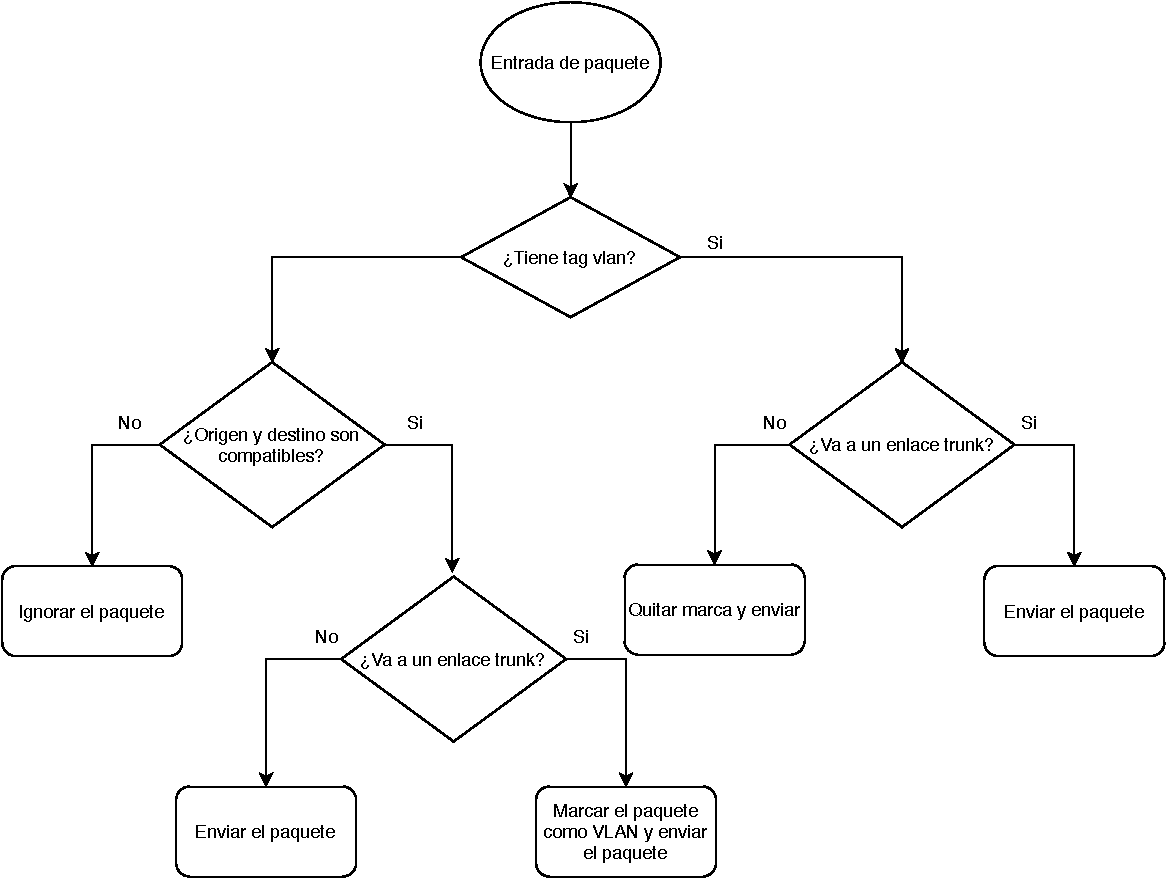
\includegraphics[width=\textwidth]{imagenes/figuras/decisiones_vlan.pdf}
    \caption{Diagrama de flujo del reenvío con VLAN}
    \label{fig:decisiones-vlan1}
\end{figure}

Empezamos creando una clase que nos permita saber a que VLAN pertenece cada nodo en función de su dirección MAC. La clase creada es la siguiente:

\begin{lstlisting}[language=Python, label=lst:vlan-assigner, caption={Clase encargada de determinar a que VLAN pertenece un nodo}]
class VlanAssigner():
    def __init__(self):
        self.vlans = [10,20,30] #Vlans disponibles
        self.default_vlan = 10 # Vlan por defecto
        self.macs_wildcards = {
            10 : [ #Vlan por defecto, trafico general
                'c2:c3:ae:8e:bf:25' #Mac del servidor
            ],
            20 : [ #Vlan de seguridad
                '01:ab:*',
                'c2:c3:ae:8e:bf:25' #Mac del servidor
            ],
            30 : [ #Vlan de telefonia
                '02:cd:*',
                'c2:c3:ae:8e:bf:25', #Mac del servidor
                '48:*'
            ]
        }

    def match_vlan(self,mac):
        encontrado = False
        resultado = []

        for k,v in self.macs_wildcards.items():
            for exp in v:
                r = re.compile(exp)
                if r.match(mac):
                    encontrado = True
                    resultado.append(k)
        if not encontrado:
            resultado.append(self.default_vlan)
        
        resultado.sort()
        return resultado
\end{lstlisting}

Ahora podemos empezar a implementar la lógica de reenvío de paquetes. Un problema con el que nos encontramos es que los paquetes broadcast (sean ARP o DHCP) no pueden enviarse debido a que la red no sabe a qué nodo van dirigidos (dirección destino ff:ff:ff:ff:ff:ff) por lo que los nodos no pueden establecer conexiones entre sí (no pueden resolver su mac a partir de su ip).

Por el problema descrito anteriormente tenemos que modificar la lógica de reenvío de paquetes de la siguiente manera:

\begin{figure}[!h]
    \centering
    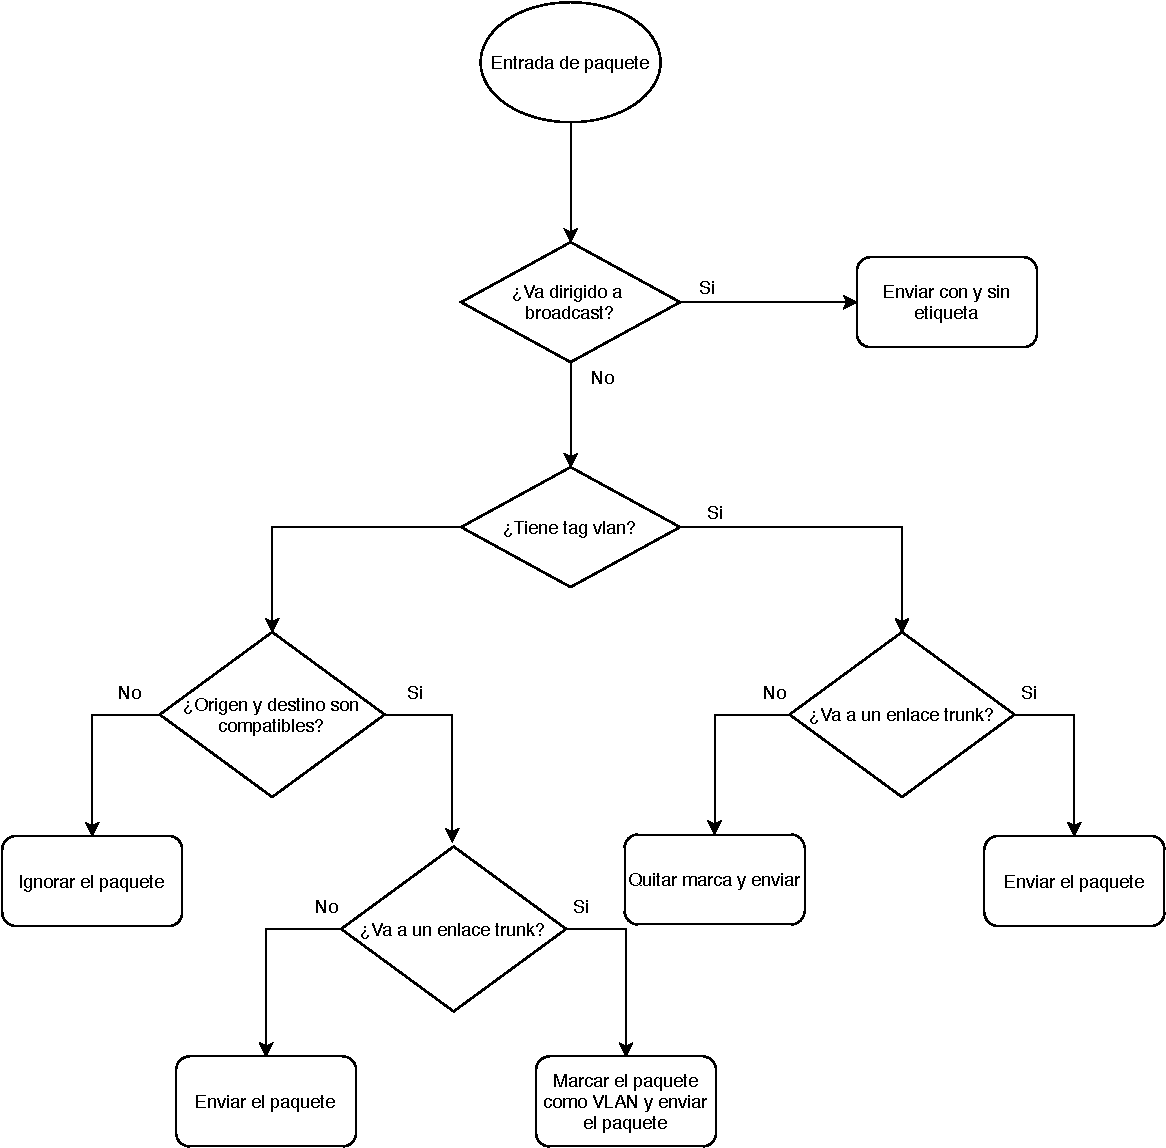
\includegraphics[width=\textwidth]{imagenes/figuras/decisiones_vlan2.pdf}
    \caption{Diagrama de flujo del reenvío con VLAN teniendo en cuenta direcciones broadcast}
    \label{fig:decisiones-vlan2}
\end{figure}

Como podemos ver en la figura \ref{fig:decisiones-vlan2} los paquetes broadcast se envían duplican: unos llevan tag VLAN y otros no. Aunque esto puede parecer un problema no lo es ya que las tarjetas de red ignoran los paquetes encapsulados en una VLAN si esta no está configurada explícitamente.

Una vez tenemos resuelto el problema de los paquetes broadcast podemos terminar de implementar la lógica de reenvío.

Si nos llega un paquete procedente de una VLAN puede venir de un host multiVLAN o de otro switch (recordemos que las decisiones de reenvío son individuales para cada switch). Tenemos que determinar primero si los host origen y destino pertenecen a la misma VLAN. Para ello hacemos uso de la siguiente función:

\begin{lstlisting}[language=Python, label=lst:vlan-compatible, caption={Función que determina si dos nodos pertenencen a la misma VlAN}]
def vlan_compatibles(self,src,dst):
    vlan_src = self.v.match_vlan(src)
    vlan_dst = self.v.match_vlan(dst)
    for v in vlan_src:
        if v in vlan_dst: return v
    return False
\end{lstlisting}

Si ambos nodos pueden comunicarse entre ellos enviamos el paquete al puerto donde sabemos que se encuentra el nodo (o el switch que se comunica con el nodo). Tenemos que discernir entre si estamos enviando a un puerto trunk o a un puerto de acceso. Como esto no lo sabemos a priori hacemos uso de la api de descubrimiento de topología de ryu. Si es un puerto trunk enviamos el paquete tal como nos ha entrado. Si es un puerto de acceso quitamos las marcas de VLAN mediante la acción \lstinline{OFPActionPopVlan()} de OpenFlow 1.3 y enviamos el paquete. Si no sabemos a que puerto tenemos que enviar el paquete (porque no conocemos todavía en nuestro switch al destinatario) enviamos el paquete por todos los puertos disponibles. Si conocemos al destinatario y el paquete se puede enviar instalamos una nueva regla de reenvío en el switch de forma que el próximo paquete dirigido a dicho nodo destino por la misma VLAN sea reenviado de forma transparente por el switch sin tener que volver a ejecutar este algoritmo en el controlador.

En caso que nos llegue un paquete sin marca de VLAN seguimos un proceso similar al anteriormente descrito pero añadiendo mediante la instrucción \lstinline{OFPActionPushVlan()} de OpenFlow su correspondiente marca.

Todo el código puede ser consultado en el repositorio del trabajo en el archivo controlador\_vlan.py.

\subsection{Descubrimiento de topología}

Para poder determinar si un puerto es trunk o no tenemos que saber donde está conectado: si está conectado a un nodo final es un puerto de acceso, si lo está a otro switch es un puerto trunk (entre switches todos los paquetes viajan taggeados). Para eso vamos a hacer uso de la api de descubrimiento de topología de Ryu que, mediante intercambio de paquetes de tipo \acrshort{lldp} \footnote{Link Layer Discovery Protocol, Protocolo de intercambio de información entre vecinos a nivel 2 (enlace)}, nos permite conocer la topología de nuestra red activa. De esta forma aprovechamos esta función para crear la siguiente función que determina si un puerto es trunk o de acceso:

\begin{lstlisting}[language=Python, label=lst:is-trunk, caption={Función que determina si un puerto es de tipo trunk}]
def is_trunk(self, dpid, port_no):
    links_list = get_link(self, dpid)
    links=[link.src.port_no for link in links_list]
    return (port_no in links)
\end{lstlisting}

En el código anterior la función \lstinline{get_link} nos devuelve los enlaces entre switches del switch con identificador \lstinline{dpid}.

De igual manera podemos conocer si un host pertenece a múltiples VLANs y por tanto su puerto es de tipo trunk contando a cuantas VLAN pertenece. Si es a más de una es un nodo miembro de varias VLAN y deberá recibir los paquetes marcados.


\subsection{Aplicación STP}

En la red que estamos implementando tenemos varios enlaces redundantes para asegurar la disponibilidad del sistema. Esta decisión de diseño trae un problema aparejado: tenemos que eliminar los bucles de la red para evitar el fenómeno conocido como tormenta de broadcast (véase figura  \cite{Spanning33:online}. Ryu tiene una librería integrada que implementa el protocolo STP y bloquea los puertos que hacen que haya bucles en la red.

\begin{figure}[!h]
    \centering
    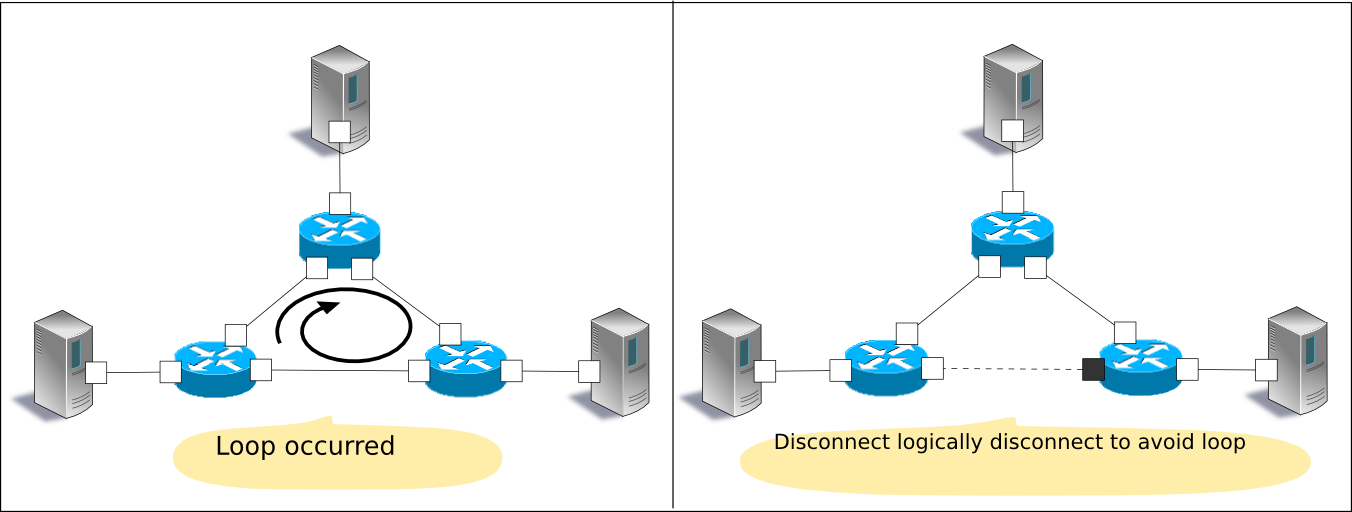
\includegraphics[width=\textwidth]{imagenes/figuras/stp.png}
    \caption{Motivación para utilizar STP. Fuente: ryu-book \cite{Spanning54:online}}
    \label{fig:motivacion-stp}
\end{figure}

Para activar el protocolo STP lo habilitamos en los contextos de nuestra aplicación

\begin{lstlisting}[language=Python, label=lst:stp-enable, caption={Activación del protocolo STP}]
_CONTEXTS = {
    'stplib': stplib.Stp
}
def __init__(self, *args, **kwargs):
    super(VlanSwitch,self).__init__(*args,**kwargs)
    self.mac_to_port = {}
    self.v = VlanAssigner()
    # Integracion de STPLib
    self.stp = kwargs['stplib']
\end{lstlisting}

Una vez hemos añadido el código indicado en \ref{lst:stp-enable} nuestra red ya ejecuta el protocolo STP. Si cae algún enlace o se activa uno nuevo el protocolo se vuelve a ejecutar de forma automática, permitiendo que la red responda dinámicamente a posibles cambios en la topología.


\section{Servicios auxiliares en el servidor}

Para poder correr la red y hacer pruebas sobre ella nos hace falta un nodo que actúe de servidor. Su tarea principal es servir direcciones mediante DHCP aunque también podría funcionar como servidor de contenido o como puerta de enlace hacia otras redes.

Lo primero que necesitamos es instalar un par de paquetes (suponiendo una distribución Linux basada en Debian)

\begin{lstlisting}[language=bash, label=lst:install-dhcp, caption={Instalación de paquetes en el servidor de la red.}]
sudo apt install vlan isc-dhcp-server
sudo modprobe 8021Q
\end{lstlisting}

\subsection{Servidor DHCP}

Además tenemos que modificar el archivo de configuración que se encuentra en \lstinline{/etc/dhcp/dhcpd.conf} para incluir una configuración similar a esta.

\begin{lstlisting}[language=bash, label=lst:dhcp-conf, caption={Configuración del servidor DHCP para servir a múltiples VLANs}]
subnet 10.0.0.0 netmask 255.255.255.0 {
  range 10.0.0.10 10.0.0.250;
  option domain-name-servers 8.8.8.8;
  option subnet-mask 255.255.255.0;
  option routers 10.0.0.1;
  option broadcast-address 10.0.0.255;
  default-lease-time 600;
  max-lease-time 7200;
  INTERFACES="router-eth0.10";
}

subnet 10.0.1.0 netmask 255.255.255.0 {
  range 10.0.1.10 10.0.1.250;
  option domain-name-servers 8.8.8.8;
  option subnet-mask 255.255.255.0;
  option routers 10.0.1.1;
  option broadcast-address 10.0.1.255;
  default-lease-time 600;
  max-lease-time 7200;
  INTERFACES="router-eth0.20";
}

subnet 10.0.2.0 netmask 255.255.255.0 {
  range 10.0.2.10 10.0.2.250;
  option domain-name-servers 8.8.8.8;
  option subnet-mask 255.255.255.0;
  option routers 10.0.2.1;
  option broadcast-address 10.0.2.255;
  default-lease-time 600;
  max-lease-time 7200;
  INTERFACES="router-eth0.30";
}
\end{lstlisting}

Con la configuración mostrada en el listado \ref{lst:dhcp-conf} conseguimos que el servidor DHCP escuche y atienda peticiones por todas las VLANs.

\section{Despliegue}

Una vez tenemos todo implementado y el servidor preparado procedemos a ejecutar el controlador y la red. Los pasos a seguir son los siguientes:

\subsection{Instalación de Mininet y Ryu}

En un entorno Linux basado en Ubuntu con python3 instalado ejecutamos los siguientes comandos para instalar Mininet-wifi y Ryu.

\begin{lstlisting}[language=bash, label=lst:install, caption={Instalación de Mininet-wifi y Ryu}]
git clone https://github.com/intrig-unicamp/mininet-wifi
cd mininet-wifi
sudo util/install.sh -Wlnfv
sudo pip install ryu
\end{lstlisting}

\subsection{Simulación de la red y ejecución del controlador}

Ahora podemos arrancar nuestra red virtualizada para hacer pruebas. Para ello tenemos que abrir dos consolas distintas.

\begin{enumerate}
    \item En la primera consola ejecutamos para arrancar el controlador Ryu:

\lstinline{sudo ryu-manager controlador_vlan.py --observe-links}

    \item En la segunda consola ejecutamos el script de topología de Mininet:

\lstinline{sudo python topologia_oficina.py}
\end{enumerate}

Teniendo estas dos consolas activas ya tenemos nuestra red funcionando. Desde la consola donde hemos ejecutado mininet podemos acceder a terminales de cada uno de los nodos de la red, así como ejecutar wireshark para hacer capturas de paquetes en cualquiera de los enlaces de la red.

\begin{figure}[!h]
    \centering
    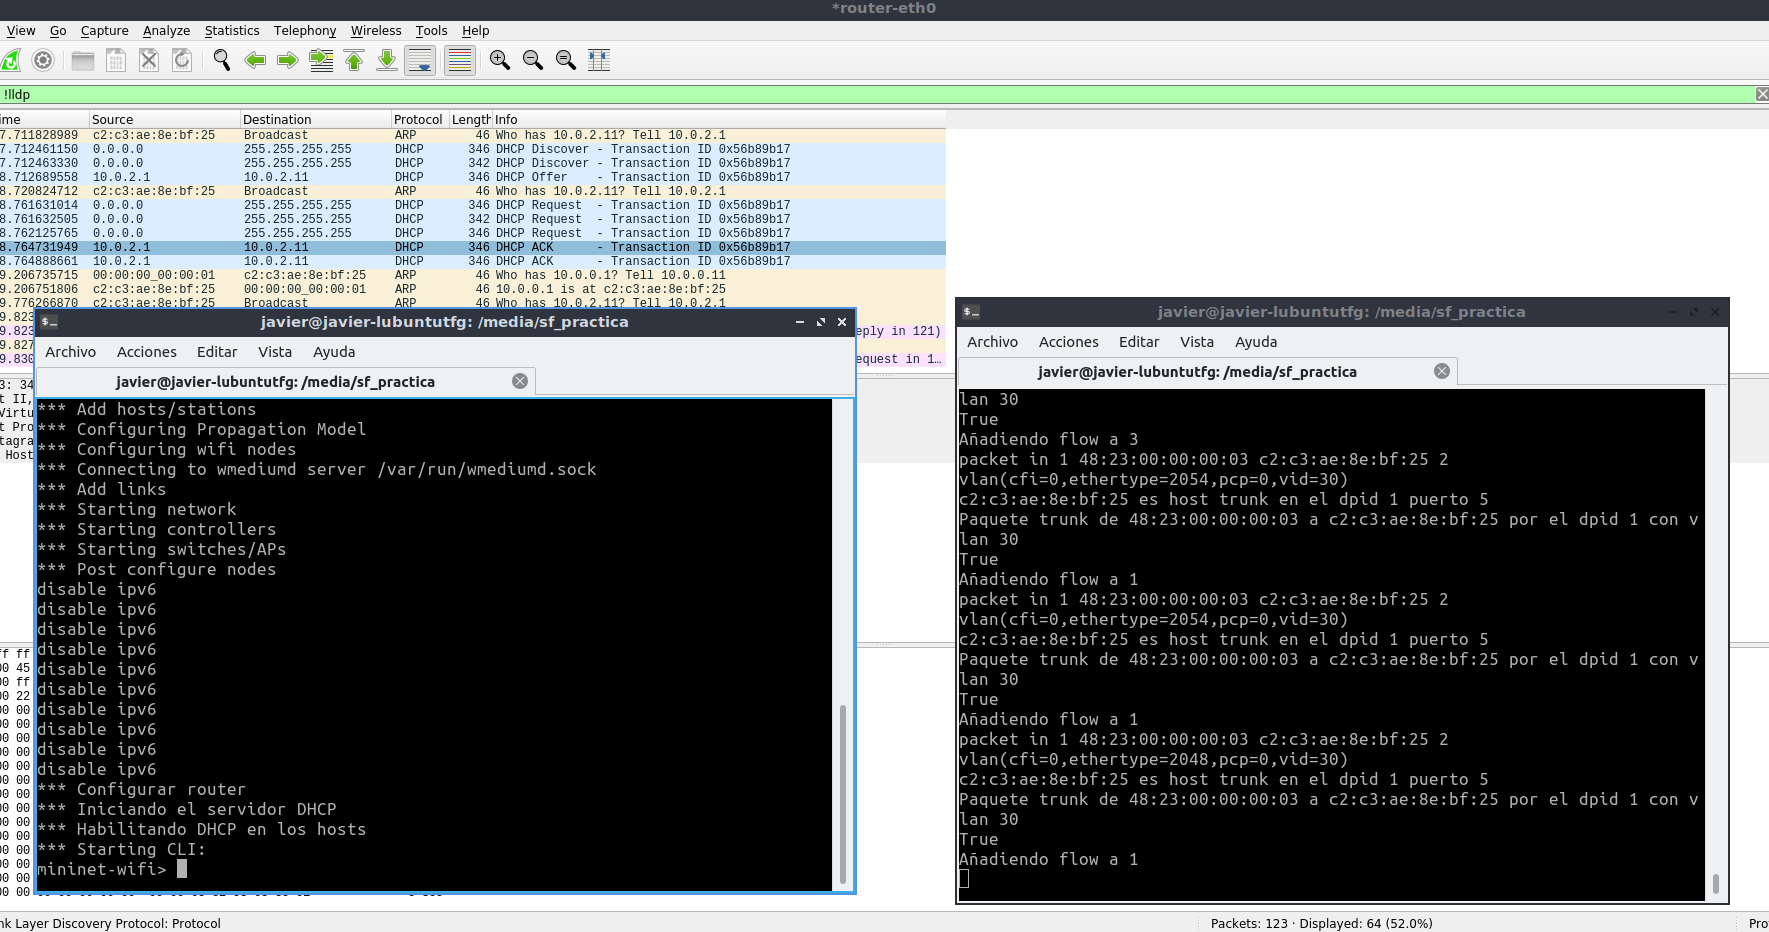
\includegraphics[width=\textwidth]{imagenes/figuras/red_funcionando.png}
    \caption{Red en funcionamiento con wireshark de fondo mostrando los paquetes que llegan al router.}
    \label{fig:red-funcionando}
\end{figure}

%
\chapter{Evaluación de la red}
%\todo{evaluación de las red? Vamos a testear las funciones uqe has creado... DONE: Mejor que pruebas, si.}

Una vez que tenemos nuestra red funcionando y le hemos dado unos segundos para configurarse automáticamente vamos a realizar algunas pruebas sobre la misma para comprobar que la funcionalidad que hemos implementado funciona correctamente.

\section{Autoconfiguración de equipos.}

Vamos a probar que los nodos se autoconfiguran de forma automática como habíamos planeado. Para comprobar esto, al arrancar la red ejecutamos el comando \lstinline{ifconfig} en uno de los hosts de la red. Al principio aparece que no tiene asociada una dirección IP. Al cabo de unos segundos cuando la red ha convergido y ha dado tiempo a intercambiar todos los paquetes necesarios los hosts tienen dirección IP.

\begin{figure}[!h]
    \centering
    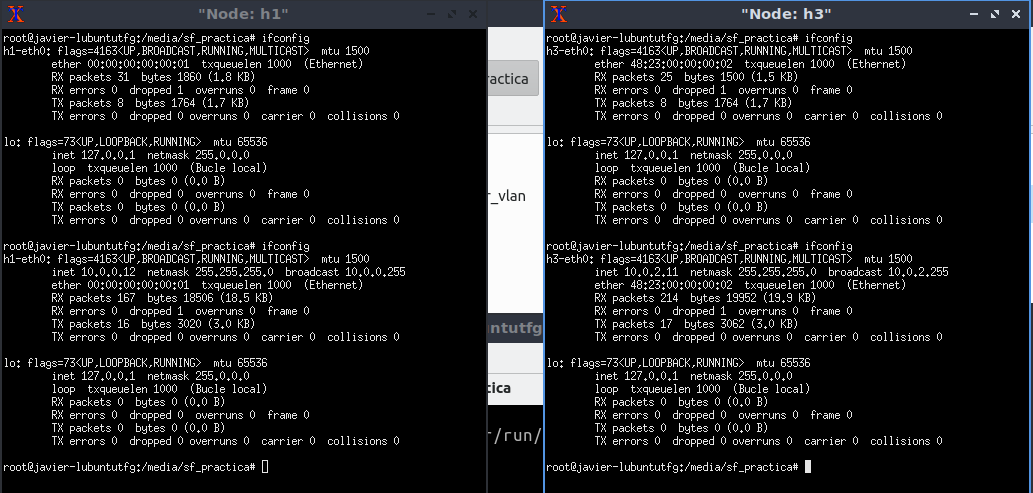
\includegraphics[width=\textwidth]{imagenes/figuras/autoconfig.png}
    \caption{Consolas de los nodos h1 y h3, pertenecientes a VLAN distintas mostrando su configuración al inicio y tras obtener una dirección IP}
    \label{fig:autoconfig}
\end{figure}

Como podemos observar en la figura \ref{fig:autoconfig} los nodos de la red obtienen del servidor DHCP una dirección IP en base a la VLAN a la que pertenecen. 

\section{Caída de enlaces}

Para comprobar la resiliencia de la red ante caídas de enlace y el correcto funcionamiento del protocolo STP vamos a probar a desactivar un enlace y hacer ping entre un nodo y el router.

\begin{figure}[!h]
    \centering
    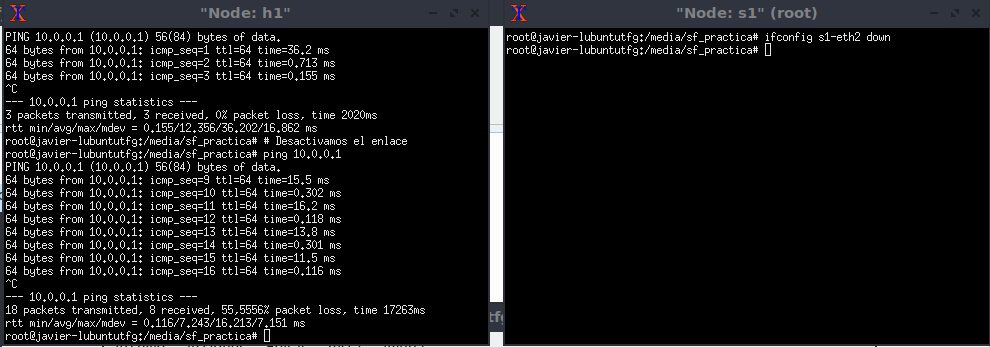
\includegraphics[width=\textwidth]{imagenes/figuras/caida_enlace.png}
    \caption{Ping entre dos dispositivos en un escenario de enlace caído}
    \label{fig:caida-enlace}
\end{figure}

Según se observa en la captura \ref{fig:caida-enlace} desconectamos una interfaz de red que conecta el switch 1 con el switch 3. El nodo es capaz de seguir accediendo al servidor a pesar del enlace caído ya que la red vuelve a ejecutar el algoritmo STP para eliminar bucles y conseguir conectividad completa de la red siempre que sea posible. En una red redundante como la que hemos diseñado tienen que caer todos los enlaces de un switch para que este se quede aislado del resto de la red.


\section{Evaluación de prestaciones}

Vamos a medir 3 parámetros básicos: la latencia media entre dispositivos, el retardo del primer paquete entre dos nodos y la velocidad pico alcanzable. Estas medidas serán ideales ya que nos encontramos en una red virtualizada. En un entorno real estas medidas pueden variar.

\subsection{Latencia media entre dispositivos}

Para conocer la latencia media de una manera aproximada vamos a ejecutar nmap desde el router dándole la orden de ejecutar pings a todos los dispositivos de la red. La línea a ejecutar es la siguiente:
\lstinline{nmap -sn 10.0.0,2.10-15} y su salida es esta:

\begin{lstlisting}[language=bash, label=lst:nmap-out, caption={Salida de nmap}]
root@javier-lubuntutfg:/media/sf_practica# nmap -sn 10.0.0,2.10-15
Nmap scan report for 10.0.0.10
Host is up (0.011s latency).
Nmap scan report for 10.0.0.11
Host is up (0.044s latency).
Nmap scan report for 10.0.0.12
Host is up (0.073s latency).
Nmap scan report for 10.0.2.10
Host is up (0.038s latency).
Nmap scan report for 10.0.2.11
Host is up (0.038s latency).
Nmap done: 12 IP addresses (5 hosts up) scanned in 26.83 seconds
\end{lstlisting}

Del listado \ref{lst:nmap-out} podemos aproximar una latencia media de 40,8 ms. Como nos parece mucho ping para una red local probamos a hacer pings individuales y hacer la media de las medias de ping. Lo hemos ejecutado con estos parámetros \lstinline{ping -q -c10 10.0.X.X}

\begin{lstlisting}[language=bash, label=lst:ping-out, caption={Salida de ping}]
root@javier-lubuntutfg:/media/sf_practica# ping 10.0.2.10 -q -c 10
--- 10.0.2.10 ping statistics ---
10 packets transmitted, 10 received, 0% packet loss, time 9198ms
rtt min/avg/max/mdev = 0.138/0.228/0.414/0.093 ms
--- 10.0.2.11 ping statistics ---
10 packets transmitted, 10 received, 0% packet loss, time 9174ms
rtt min/avg/max/mdev = 0.117/0.356/1.871/0.506 ms
--- 10.0.0.10 ping statistics ---
10 packets transmitted, 10 received, 0% packet loss, time 9183ms
rtt min/avg/max/mdev = 0.077/0.243/0.909/0.228 ms
--- 10.0.0.11 ping statistics ---
10 packets transmitted, 10 received, 0% packet loss, time 9184ms
rtt min/avg/max/mdev = 0.056/0.514/3.583/1.025 ms
--- 10.0.0.12 ping statistics ---
10 packets transmitted, 10 received, 0% packet loss, time 9030ms
rtt min/avg/max/mdev = 2.368/3.567/6.754/1.263 ms
\end{lstlisting}

Del listado anterior calculamos una \textbf{latencia media de 0,978 ms}. Véase además como es el último nodo el que ralentiza más la red. Comprobando la tabla de macs sabemos que ese es el nodo que simula estar conectado mediante un enlace inalámbrico. Además mininet-wifi simula una red wifi de tipo 802.11g, de tecnología bastante más antigua que el estándar actual 802.11.ac

\subsection{Tiempo para el primer paquete}

Observando los resultados anteriores vemos que hay paquetes de ping con una latencia muy superior a la media. observando una salida completa de ping entre dos nodos que no se han comunicado entre sí anteriormente (figura \ref{fig:ping-first}) podemos comprobar que el primer paquete tarda más tiempo en llegar. Esto se debe a que el primer paquete es procesado por el controlador de la red, mientras que los paquetes sucesivos ya tienen una regla coincidente en los switches y no tienen que pasar por el controlador.

\begin{figure}[!h]
    \centering
    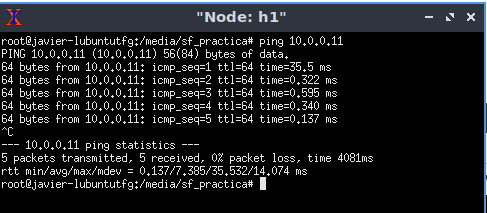
\includegraphics[width=\textwidth]{imagenes/figuras/ping_first.png}
    \caption{Ping entre dos dispositivos que no han tenido comunicación directa previamente.}
    \label{fig:ping-first}
\end{figure}

\subsection{Ancho de banda entre dos dispositivos}

Si ejecutamos iperf entre dos dispositivos podemos ver la velocidad del enlace entre ellos. En este caso vamos a medir la velocidad de enlace entre h3 y el router.

\begin{figure}[!h]
    \centering
    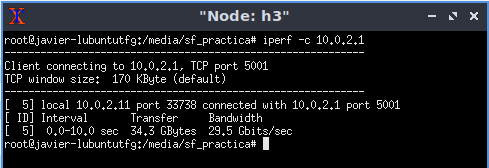
\includegraphics[width=\textwidth]{imagenes/figuras/iperf.png}
    \caption{Iperf ejecutándose entre dos nodos de la red.}
    \label{fig:iperf}
\end{figure}

La herramienta ha dado una velocidad entre ambos equipos de \textbf{29,5 Gb/s}. Esto se debe a que estamos en una red virtualizada. De hecho si probamos a hacer esta misma prueba con alguno de los nodos conectados mediante wifi veremos que alcanzamos una velocidad máxima del enlace inalámbrico (figura \ref{fig:iperf-wifi}) mucho menor: \textbf{9,65Mb/s}

\begin{figure}[!h]
    \centering
    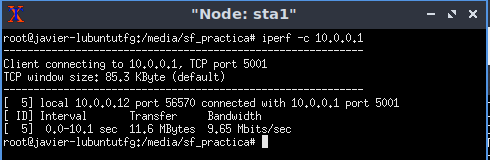
\includegraphics[width=\textwidth]{imagenes/figuras/iperf-wifi.png}
    \caption{Iperf ejecutándose entre dos nodos de la red, uno de ellos conectado de forma inalámbrica.}
    \label{fig:iperf-wifi}
\end{figure}

Medir parámetros básicos: latencia, tiempo al primer paquete, throughput medio.

%

%
\chapter{Conclusiones}

En este trabajo hemos logrado implementar con éxito una red autoconfigurable mediante Ryu. La red es capaz de detectar los dispositivos que tiene conectados y adaptar sus tablas de encaminamiento a dichos dispositivos. Además es capaz de asignar de forma dinámica una VLAN a cada nodo en el momento de conectarse basado en su dirección MAC sin la necesidad de intervención externa.

La red también es redundante en enlaces y es capaz de recuperar la conectividad de manera automática en caso de conexión de una caída de enlace.

Tras haber hecho un estudio exhaustivo de la arquitectura de redes definidas por software y haber desarrollado una podemos afirmar que, aunque la carga de trabajo a la hora de instalar la red sea grande esta facilita enormemente la administración y el mantenimiento de la misma, con su correspondiente mejora en eficacia y reducción de costes.

Como trabajo futuro se deja la inclusión de un sistema de Calidad de Servicio basado en las colas de prioridad de las que disponen los switches OpenFlow o la inclusión de un protocolo de \textit{link aggregation}.

En definitiva tenemos un proyecto software que puede ser usado, con algunos ligeros ajustes en entornos SDN reales.
%
%\input{capitulos/07_Pruebas}
%
%\input{capitulos/08_Conclusiones}
%
%%\chapter{Conclusiones y Trabajos Futuros}
%
%
\nocite{*}
\bibliography{bibliografia}\addcontentsline{toc}{chapter}{Bibliografía}
\bibliographystyle{plain}
%
%\appendix
%\input{apendices/manual_usuario/manual_usuario}
%%\input{apendices/paper/paper}

\addcontentsline{toc}{chapter}{Glosario}
\printglossary[type=\acronymtype]
\chapter*{}
\thispagestyle{empty}

\end{document}
